% bristolthesis template.tex file
% Best not to fiddle with this much/at all or things might break
% This needs to line up with the contents of bristolthesis.cls and vice versa
%
%
%
%
%

\documentclass[11pt,twoside]{bristolthesis}

%% Packages - these are those which i used for my thesis so might not be specific to yours
\usepackage{graphicx,latexsym}
\usepackage{amsmath}
\usepackage{amssymb}
\usepackage{amsthm}
\usepackage{longtable}
\usepackage{booktabs}
\usepackage{setspace}
\usepackage{siunitx}
% \usepackage{chemarr} %% Useful for one reaction arrow, useless if you're not a chem major
\usepackage[hyphens]{url}
\usepackage{hyperref}
\usepackage{lmodern}
\usepackage{float}
\floatplacement{figure}{H}
\usepackage{rotating}
% \usepackage{times} % other fonts are available like times, bookman, charter, palatino

%% Paramaters for global document
\hypersetup{colorlinks = false}
\renewcommand{\UrlBreaks}{\do\/\do\a\do\b\do\c\do\d\do\e\do\f\do\g\do\h\do\i\do\j\do\k\do\l\do\m\do\n\do\o\do\p\do\q\do\r\do\s\do\t\do\u\do\v\do\w\do\x\do\y\do\z\do\A\do\B\do\C\do\D\do\E\do\F\do\G\do\H\do\I\do\J\do\K\do\L\do\M\do\N\do\O\do\P\do\Q\do\R\do\S\do\T\do\U\do\V\do\W\do\X\do\Y\do\Z\do\0\do\1\do\2\do\3\do\4\do\5\do\6\do\7\do\8\do\9\do\%\do\.\do\-}
\renewcommand{\chapterautorefname}{Chapter}
\usepackage{times} % other fonts are available like times, bookman, charter, palatino
\usepackage{caption}

% Use ref for internal links
\renewcommand{\hyperref}[2][???]{\autoref{#1}}
\def\chapterautorefname{Chapter}
\def\sectionautorefname{Section}
\def\subsectionautorefname{Subsection}
\usepackage{caption}
\captionsetup{width=5in}

% Syntax highlighting #22
%%%

%%% YAML header functions
\title{I made this template based on thesisdown to comply with the University of Bristol regulations}
\author{Thomas Battram}
\date{September 2020}
\university{University of Bristol}
\faculty{Health Sciences}
\school{Bristol Medical School}
\group{MRC Integrative Epidemiology Unit}
\wordcount{}
\degree{Population Health Sciences}
\logo{figure/index/UoBcrest.pdf}
%%%


%%% The document formatting
\makeatletter
\def\maxwidth{ %
  \ifdim\Gin@nat@width>\linewidth
    \linewidth
  \else
    \Gin@nat@width
  \fi
}
\makeatother

\renewcommand{\contentsname}{Table of Contents}

\setlength{\parskip}{14truept}

  \setlength{\parskip}{\baselineskip}
  \usepackage[parfill]{parskip}

\providecommand{\tightlist}{%
  \setlength{\itemsep}{0pt}\setlength{\parskip}{0pt}}

\Acknowledgements{
THIS IS WHERE YOU THANK PEOPLE!!!!!!!!!!!!!!!!!!!!!!!!!!!!!!!!!!!!!!!!!!!!!!!!!!!!!!!!!!!!!!!!!
}

\Declaration{
I declare that the work in this dissertation was carried out in accordance with the requirements of the University's Regulations and Code of Practice for Research Degree Programmes and that it has not been submitted for any other academic award. Except where indicated by specific reference in the text, the work is the candidate's own work. Work done in collaboration with, or with the assistance of, others, is indicated as such. Any views expressed in the dissertation are those of the author.

\bigskip
\bigskip
\bigskip
\bigskip
\bigskip

Signed

\bigskip
\bigskip
\bigskip
\bigskip
\bigskip

Dated
}

\Abstract{
My abstract will go here and it will be a solid abstract. Full of the things that go in abstracts. Such as numbers, acronyms, other words, and lots of punctuation.

It will have multiple paragraphs too!
}

\Abbreviations{
\textbf{EWAS} - epigenome-wide assoctation study
\textbf{GWAS} - genome-wide assoctation study
\textbf{h<sup>2</sup>} - narrow-sense heritability
\textbf{h<sup>2</sup><sub>SNP</sub>} - SNP-heritability
\textbf{H<sup>2</sup>} - broad-sense heritability
\textbf{MR} - Mendelian randomization
\textbf{mQTL} - methylation quantitative trait loci
\textbf{SNP} - single nucleotide polymorphism
}

	\usepackage{tikz} \usepackage{booktabs} \usepackage{longtable} \usepackage{siunitx} \pagestyle{plain}
	\usepackage{booktabs}
 \usepackage{longtable}
 \usepackage{array}
 \usepackage{multirow}
 \usepackage{wrapfig}
 \usepackage{float}
 \usepackage{colortbl}
 \usepackage{pdflscape}
 \usepackage{tabu}
 \usepackage{threeparttable}
 \usepackage{threeparttablex}
 \usepackage[normalem]{ulem}
 \usepackage{makecell}
 \usepackage{xcolor}


\newlength{\cslhangindent}
\setlength{\cslhangindent}{1.5em}
\newenvironment{cslreferences}%
  {\setlength{\parindent}{0pt}%
  \everypar{\setlength{\hangindent}{\cslhangindent}}\ignorespaces}%
  {\par}


%%% Main document
\spacing{1}
\begin{document}
  \maketitle

\frontmatter % this stuff will be roman-numbered
\pagestyle{empty} % this removes page numbers from the frontmatter
  \begin{abstract}
    My abstract will go here and it will be a solid abstract. Full of the things that go in abstracts. Such as numbers, acronyms, other words, and lots of punctuation.

    It will have multiple paragraphs too!
  \end{abstract}
  \begin{acknowledgements}
    THIS IS WHERE YOU THANK PEOPLE!!!!!!!!!!!!!!!!!!!!!!!!!!!!!!!!!!!!!!!!!!!!!!!!!!!!!!!!!!!!!!!!!
  \end{acknowledgements}
  \begin{declaration}
    I declare that the work in this dissertation was carried out in accordance with the requirements of the University's Regulations and Code of Practice for Research Degree Programmes and that it has not been submitted for any other academic award. Except where indicated by specific reference in the text, the work is the candidate's own work. Work done in collaboration with, or with the assistance of, others, is indicated as such. Any views expressed in the dissertation are those of the author.

    \bigskip
    \bigskip
    \bigskip
    \bigskip
    \bigskip

    Signed

    \bigskip
    \bigskip
    \bigskip
    \bigskip
    \bigskip

    Dated
  \end{declaration}
  \hypersetup{linkcolor=black}
  \setcounter{tocdepth}{3}
  \tableofcontents
  \listoftables
  \listoffigures

\spacing{1.5}
\mainmatter % here the regular arabic numbering starts
\pagestyle{plain}
\hypertarget{preface}{%
\chapter*{Preface}\label{preface}}
\addcontentsline{toc}{chapter}{Preface}

This template is based on (and in many places copied directly from) the Reed College LaTeX template, but hopefully it will provide a nicer interface for those that have never used TeX or LaTeX before. Using \emph{R Markdown} will also allow you to easily keep track of your analyses in \textbf{R} chunks of code, with the resulting plots and output included as well. The hope is this \emph{R Markdown} template gets you in the habit of doing reproducible research, which benefits you long-term as a researcher, but also will greatly help anyone that is trying to reproduce or build onto your results down the road.

Hopefully, you won't have much of a learning period to go through and you will reap the benefits of a nicely formatted thesis. The use of LaTeX in combination with \emph{Markdown} is more consistent than the output of a word processor, much less prone to corruption or crashing, and the resulting file is smaller than a Word file. While you may have never had problems using Word in the past, your thesis is likely going to be about twice as large and complex as anything you've written before, taxing Word's capabilities. After working with \emph{Markdown} and \textbf{R} together for a few weeks, we are confident this will be your reporting style of choice going forward.

\textbf{Why use it?}

\emph{R Markdown} creates a simple and straightforward way to interface with the beauty of LaTeX. Packages have been written in \textbf{R} to work directly with LaTeX to produce nicely formatting tables and paragraphs. In addition to creating a user friendly interface to LaTeX, \emph{R Markdown} also allows you to read in your data, to analyze it and to visualize it using \textbf{R} functions, and also to provide the documentation and commentary on the results of your project. Further, it allows for \textbf{R} results to be passed inline to the commentary of your results. You'll see more on this later.

\textbf{Who should use it?}

Anyone who needs to use data analysis, math, tables, a lot of figures, complex cross-references, or who just cares about the final appearance of their document should use \emph{R Markdown}. Of particular use should be anyone in the sciences, but the user-friendly nature of \emph{Markdown} and its ability to keep track of and easily include figures, automatically generate a table of contents, index, references, table of figures, etc. should make it of great benefit to nearly anyone writing a thesis project.

\textbf{For additional help with bookdown}
Please visit \href{https://bookdown.org/yihui/bookdown/}{the free online bookdown reference guide}.

\hypertarget{introduction}{%
\chapter{Introduction}\label{introduction}}

This thesis focuses on epigenome-wide association studies (EWAS), which assess the association between DNA methylation changes throughout the genome and traits of interest. Advances in technology and an increasing number of samples has lead to hundreds of EWAS having been performed to date (more details in \textbf{Chapter \ref{ewas-catalog}}). Goals of these EWAS have included using DNA methylation marks to use as predictors, diagnostic factors, and modifiable mediators of traits.

To help inform design of future studies, there is a need to understand what has been discovered thus far in EWAS and what future EWAS are likely to add in the context of current EWAS and other study designs. Further, to improve biological inference of sites identified in EWAS, causality (or lack of) should be established.

Some key elements which are not currently understood:
\begin{itemize}
\tightlist
\item
  Why certain DNA methylation sites/regions of the genome are more prevalent in EWAS to date. Could this be because of genuine biological importance of these sites or because of some technical artefact?
\item
  How much trait variation DNA methylation tends to associate with and thus how much more information there is to gain from EWAS of greater sample sizes
\item
  Whether EWAS can add to current biological understanding above what can be learnt from other study designs
\item
  Whether DNA methylation-trait associations in EWAS are likely to be causal
\end{itemize}
In this chapter I describe DNA methylation in context of the regulatory processes in human cells, discuss it's potential for use in population level studies and describe the current state of EWAS research. Then I discuss how epigenetic-epidemiologists can draw on the methods developed by geneticists to 1. understand what information has been gained from EWAS, 2. understand what information is left to gain from EWAS and 3. understand the causal nature of DNA methylation-trait associations identified in EWAS.

\hypertarget{dna-methylation-as-part-of-the-regulome}{%
\section{DNA methylation as part of the regulome}\label{dna-methylation-as-part-of-the-regulome}}

DNA methylation is one of many epigenetic marks that are involved in gene regulation (the regulome), so here I briefly outline some of these regulatory marks and discuss DNA methylation in the context of this complex biological process.

\hypertarget{the-regulome}{%
\subsection{The regulome}\label{the-regulome}}

Gene expression is a tightly controlled process and only in the right circumstances will RNA polymerase II be able to bind the correct site, initiate and finally complete the transcription process (REFS). The importance of this level of control is no more apparent than in the developmental stages of human life. Humans start as a single cell and after roughly nine months are transformed into a multicellular organism with trillions of cells, including hundreds of unique cell types (REF). As these cells arise from a single progenitor they must contain identical genetic sequences (except a few somatic mutations). Therefore, the process by which the body is able to create such diversely functioning cells and tissues, must come from regulation of how the genetic sequence is read and regulation of its products (REFs). Indeed it was in developmental biology that we first began to understand the processes that may regulate gene expression (REFs). There are a plethora of methods cells use to regulate gene and protein expression post-transcriptionally (REFs), but these are beyond the scope of this thesis. So I'll continue to describe the regulome just in the context of epigenetic marks.

\hypertarget{defining-epigenetics}{%
\subsection{Defining epigenetics}\label{defining-epigenetics}}

The definition of epigenetics is much debated amongst those who study cellular and molecular processes (REFs). In the 1940s the `epigenetic landscape' was introduced by Waddington to describe how genes influence cell fates (Stern C.D, 2000 - Waddington's contributions to avian and mammalian development). Since then the term epigenetics has been used in many forms, so to avoid confusion, throughout the rest of the thesis, here is what I mean when using the term \textbf{epigenetics}: the study of mitotically heritable changes in gene expression that occur without changes in DNA sequence. When referring to \textbf{epigenetic marks} I simply mean chemical changes to the genome and genome-bound proteins that are mitotically heritable and may influence gene expression without changing the DNA sequence.

\hypertarget{histone-modifications}{%
\subsection{Histone modifications}\label{histone-modifications}}

Histones are genome-bound proteins composed of four subgroups that are present twice each in a single histone octamer. Modifications can occur to any of the histone monomers and these have been associated with both positive and negative changes in gene expression (REFs). Histone modifications are numerous and complex in nature. To briefly describe the complexity, there are at least \textbf{X} types of histone modifications, each of the histone monomers can be modified across many different sites, and for any one site mutiple of the same modification can occur. It is the combination of all of this that plays a role in gene expression regulation (REFs). Furthermore, histone modifications are subject to rapid change upon environmental stimulus to help induce or repress gene expression (REFs). Consequently, functions of only a few histone marks have been reliably established thus far (REFs) and taking a snapshot of the histone modifications present in cells may give a poor summary of how gene regulation is occurring. Very few population-based studies have assessed histone modifications because of these, plus some other technical difficulties (REFs). They may become far more prominent in the future as our understanding and ability to measure the modifications in a meaningful way increases.

\hypertarget{dna-methylation}{%
\subsection{DNA methylation}\label{dna-methylation}}

Good review: Peter Jones 2012
DNA methylation is the addition of a methyl group to the DNA, which primarily occurs at the 5' cytosine of a CpG site. Little is known about the role of non-CpG site DNA methylation and current EWAS tend to only measure CpG methylation, so that will be my focus here. The function of this epigenetic mark was proposed back in 1975 (REFs), where two papers suggested it represses gene expression and ever since then many papers have shown the correlation between DNA methylation at gene promoters and a reduction in expression of those genes (REFs). Unfortunately, it's not that simple and even now the role of DNA methylation is being debated, with a paper recently suggesting that any DNA methylation changes associated with alterations in gene expression were just a by-product of other regulatory processes such as transcription factor binding (REF). Regardless, DNA methylation is closely linked with genomic function and correlates with various aspects in different ways, as depicted in \textbf{Figure \ref{fig:dnam-fig}}.

CpG sites are not randomly distributed throughout the genome (REF), but are often found in clusters and so if DNA methylation does have an effect on processes like gene expression regulation it's thought that methylation and de-methylation of CpG sites in groups is what drives their regulatory function. To support this, there are clear biological processes that regulate DNA methylation at nearby sites together, for example, CpG sites at transcription factor binding sites will be de-methylated as a group when the transcription factor binds (REF). Further nearby sites are often statistically correlated, suggesting regulation as a group. However, there is no evidence to suggest that neighbouring sites do indeed act in tandem or whether it is likely one site from the group is driving regulatory function. This is something I explore in (\textbf{Chapter \ref{h2ewas-chapter}}).

One major difference between DNA methylation and other epigenetic marks, that was alluded to earlier, is that DNA methylation is far more stable. Enzymes do exist that can actively de-methylate the DNA, for example the ten-eleven translocation (TET) enzymes, but ultimately cell division is required for full de-methylation of a DNA molecule. Biologically, this suggests DNA methylation might be involved in long-term repression of gene expression, which can be seen for X-inactivation, and practically it makes studying the epigenetic mark easier as it prevents large temporal variations in DNA methylation (though they may occur!), so fewer samples are needed.

Figure here:

Figure should contain these diagrams:
1. DNA methylation at TSS and no DNA methylation in gene body (repressed transcription)
2. No DNA methylation at TSS and DNA methylation in gene body (active transcription)
3. DNA methylation in centromeres
4. DNA methylation at transposable elements

\hypertarget{dnam-phs}{%
\section{Use of DNA methylation in a population setting~}\label{dnam-phs}}

The importance of DNA methylation to disease has already been established in rare developmental disorders caused by aberrant imprinting patterns (REF), but the focus of this thesis is on studying DNA methylation in relation to complex phenotypes. In this section I discuss the appeal of studying DNA methylation in this context, introduce the most common study design for doing so, EWAS, and discuss successes and complications of the work.

\hypertarget{appeal-of-dnam}{%
\subsection{The appeal of DNA methylation to epidemiologists}\label{appeal-of-dnam}}

All epigenetic modifications are of potential interest to those studying any phenotype. Arguably, epigenetics could underlie all phenotypic changes and be the difference between individuals who develop disease and those who don't (REF). Further, epigenetic marks are modifiable, which means theoretically it would be possible to prevent or treat any disease by altering the epigenetic patterns of individuals (REF). As will be discussed in \protect\hyperlink{problems-for-ewas}{Problems for EWAS}, there are large practical problems to this. Even if targeting epigenetic marks is not easy, as long as it is possible to observe them they could be used as diagnostic biomarkers and predictors (REF). Thus, the ability to measure, and the research in to understanding epigenetic mechanisms could have broad consequences for public health (REF). As mentioned, DNA methylation is more stable than other epigenetic marks making it easier to measure on a large scale, leading to it being the epigenetic mark of choice to study in larger samples. Also, as alluded to, the regulatory processes that all govern whether genes are transcribed are linked, making DNA methylation highly correlated with other epigenetic marks (REFs), known examples included positive correlation with the histone modification H3K9me3 (REFs) and negative correlation with histone acetylation (REFs). This means measuring DNA methylation may capture more than just the one epigenetic mark and recently it's been shown that epigenetic marks can be used to predict each other with high accuracy (REF).

\hypertarget{ewas}{%
\subsection{Epigenome-wide association studies}\label{ewas}}

EWAS are the most common study design for assessing the association between DNA methylation and a complex trait (REF). They typically involve measuring hundreds of thousands of DNA methylation sites across the genome in a case-control or cohort setting and using linear models to assess the association between DNA methylation and the trait of interest. It's a study design that has been widely adopted over the past ten years and the relationship between a plethora of traits, from smoking to anthropometric measures to childhood adversities, and DNA methylation has now been studied (REFs). There are also large consortia that are pooling samples to gain power for these studies, for example the Pregnancy and Epigenetics Consortium (PACE) (REF). One clear success in EWAS is with the study of smoking. DNA methylation across thousands of sites have been shown to be associated with smoking (REF) and for many of these sites this has been replicated (REF). DNA methylation can predict smoking status, potentially better than self-report (REF). It has been revealed the direction of effect at some sights is likely from smoking to DNA methylation and in fact over time the DNA methylation changes caused by smoking may be (mostly) reversible by giving up smoking (REF). Another complex trait shown to relate to large variation in DNA methylation across the genome is age (REFs), so much so that DNA methylation makes a highly accurate predictor for age (REFs). All these studies have shown that large perturbations in the DNA methylome can be related to complex traits, and so studying DNA methylation in this fashion has huge potential.

\hypertarget{problems-for-ewas}{%
\subsection{Problems for EWAS}\label{problems-for-ewas}}

\hypertarget{confounding}{%
\subsubsection{Confounding}\label{confounding}}

Confounding, where the traits of interest share a common cause, can lead to associations between traits despite a lack of causality. Complex traits are strongly correlated with each other, often in clusters, which can lead to large amounts of measured and unmeasured confounding being present in observational epidemiological studies. As an observational design, EWAS also suffers from this problem. Of course, in order to produce therapies to prevent or treat disease by altering DNA methylation or other parts of the epigenome, causality must be established. Therefore, problems of confounding must be overcome in EWAS to use these results to start developing new drugs, this is discussed more in \protect\hyperlink{establishing-causality}{Establishing causality}.

\hypertarget{cell-type-heterogeneity}{%
\subsubsection{Cell type heterogeneity}\label{cell-type-heterogeneity}}

As discussed, epigenetic factors guide differentiation of a single pluripotent cell to hundreds of cell types in human development. As these cell types can have large differences in morphology and function, it is clear that epigenetic marks, including DNA methylation, will vary widely between cell types (REF). This poses two distinct problems for EWAS. Firstly, when collecting samples to measure DNA methylation, unless cells are purified, then a pool of cell types will be present in the samples, each with their own distinct DNA methylation patterns. This can lead to issues of confounding by cell type. For example, in a case control study, cases may be more likely to have increased numbers of CD4+ Th2 immune cells and these cells may on average have a higher level of DNA methylation at site X. In this scenario if you were to take blood cells, measure DNA methylation, and assess the association between DNA methylation and the trait of interest, you'd find an association between DNA methylation at site X and the trait, but in this is just a function of the increased number of CD4+ Th2 cells present in cases and site X has no causal relationship with the trait itself. There have been efforts to try and account for cell type heterogeneity in EWAS (REFs), but to completely prevent it's confounding effects, cells should be purified. The second problem arising from cell-type specific patterns of DNA methylation is the uncertainty that the cell type being studied is in fact one in which DNA methylation covaries with the trait of interest. Invasive cells to collect, such as blood, skin, and saliva, are common amongst epidemiological studies, but it is unclear whether EWAS in these studies are relevant to a large proportion of complex traits. This is studied, with regards to blood, in \textbf{Chapter \ref{h2ewas-chapter}}. Studies have actually shown high levels of correlation between DNA methylation of different cell types (REFs), but it is unknown whether the correlated sites are important to trait variation. Further, this correlation may complicate things with regards to epigenetic therapies. Some organs, such as the brain, are difficult to target with therapies (REF) so even if a promising epigenetic target is identified, it may be almost impossible to translate this into something clinically useful.

\hypertarget{measuring-dna-methylation}{%
\subsubsection{Measuring DNA methylation}\label{measuring-dna-methylation}}

Ideally, in every sample, DNA methylation would be measured across all sites in the genome. Unfortunately, this is not currently possible and sequencing technologies that offer something similar are often very expensive (REFs). There are three alternatives available to DNA methylation studies. Firstly, one could sequence a small portion of the genome if this section is of particular interest, however this candidate gene approach is unlikely to be profitable unless the genes targeted already have good evidence for epigenetic variation with the trait of interest (REFs). Secondly, measuring DNA methylation on long repeat sequences of the genome, such as long interspersed nuclear elements (LINEs) and short interspersed nuclear elements (SINEs), can provide estimates for global DNA methylation changes (REFs). This is useful to examine if a trait is related to large perturbations of DNA methylation across the genome, but gives little mechanistic insight into what effects these changes may be having, as methylation at functional genes is not measured. Thirdly, an array approach covering DNA methylation genome-wide at selected sites (REFs). This last approach is the most common for EWAS as it enables measurement of DNA methylation at hundreds of thousands of sites at a relatively cheap price per sample (REFs). The most commonly used array currently is the Illumina Infinium HumanMethylation450 (HM450) Beadchip, which measures DNA methylation at over 450,000 sites across the whole genome. Technology is always getting better and recently the Illumina Infinium HumanMethylationEPIC Beadchip, measuring over 800,000 sites is now being used by some studies (REFs). The arrays are designed to cover a large number of genes and have many probes in promoter regions (REF). With current biological knowledge of DNA methylation (see section \ref{dna-methylation}) this is unsurprising, but these arrays only measure roughly 1.5-4\% of all CpG sites in the genome. Further, there is no empirical evidence to show these sites covary with complex traits. This will be examined in \textbf{Chapter \ref{h2ewas-chapter}}.

Batch effects and technical artefacts can also play a large role in EWAS. There has been considerable effort made to try and mitigate these effects and methods have been developed to help correct for batch effects (REFs). Further, studies have used sequencing methods to identify potentially unreliable probes (REFs). Removal of batch effects is readily employed in EWAS, but it is unclear as to whether potentially faulty probes have given rise to an excess of EWAS signal. This information could provide more evidence of the technical issues facing EWAS and prompt extra care when conducting these studies. This is examined briefly in \textbf{Chapter \ref{properties-of-ewas}}.

\hypertarget{complexity-of-regulatory-mechanisms}{%
\subsubsection{Complexity of regulatory mechanisms}\label{complexity-of-regulatory-mechanisms}}

EWAS identify single sites in the genome for which DNA methylation variation is associated with a trait of interest. As discussed, DNA methylation at a single site will likely be correlated with DNA methylation at neighbouring sites and other nearby epigenetic marks. This makes inferring mechanism of action very difficult. Differentially methylated region (DMR) analysis is often employed, which aims to determine if multiple neighbouring sites share an association with the trait of interest in the with the same direction of effect (REFs). These give evidence to whether the sites covary similarly with the trait of interest, but don't provide evidence that the sites are acting independently or not. A simple way to view EWAS, is that they identify potentially important regions of the genome with respect to the trait of interest, i.e.~they suggest that genes in that region may be influenced by or influence the trait of interest.

\hypertarget{treatments}{%
\subsubsection{Treatments}\label{treatments}}

This is not a focus of my thesis, but for completion it is important to briefly note the complications of epigenetic-based therapies as they are an end goal of much epigenetic research. Currently there are therapies used in the clinic that target enzymes responsible for epigenetic alterations, for example DNA methyltransferase inhibitors and histone deacetylase inhibitors (REFs). They are primarily used to treat cancers (REF), but as with many cancer treatments, are very toxic. These therapies impact the epigenome globally and do not target any specific regions of the genome. This makes them highly undesirable for most diseases and as of yet there are no targeted epigenetic therapies (REF).

In summary, there is great potential for EWAS to identify sites in the genome that could be targeted for treatment, but there are several challenges still to overcome. A great importance should be placed on using the data available to inform future designs of EWAS to maximise the potential of these studies.

\hypertarget{genetics-in-ewas}{%
\section{Using methods from genetics to help inform future EWAS}\label{genetics-in-ewas}}

There is a clear corollary to EWAS in genetic epidemiology, the genome-wide association study (GWAS), which also measures markers across the whole genome and assesses whether each of these markers associates with the phenotype of interest. GWAS have been around for far longer than EWAS and a huge amount of effort has been put into understanding what information is provided by these studies, what information can be discovered by these studies and how to use these results to inform other research.

\hypertarget{gwas-catalog}{%
\subsection{The GWAS Catalog}\label{gwas-catalog}}

The GWAS Catalog is a manually curated database of publicly available GWAS data, developed by the European Bioinformatics Institute (EBI) and made openly available to the public (REFs). It has a broad range of applications for researchers, from replication of GWAS, to identifying overlapping GWAS signals between traits, to pooling the data to try and understand the genetic architecture of complex traits as a whole. Resources like this are invaluable to the genetic epidemiologist community and so developing a corollary database for EWAS may provide equal opportunity for epigenetic epidemiologists. Catalogs such as EWASdb (REF) and the EWAS Atlas (REF) are currently available, but fall short of some key researcher requirements including ease of use and access to full summary statistics. The development of a new database, The EWAS Catalog, is the focus of \textbf{Chapter \ref{ewas-catalog}}.

\hypertarget{heritability}{%
\subsection{Total variance captured by all sites measured genome-wide}\label{heritability}}

Before spending lots of time and resources on measuring the relationship between traits, it's important to have an understanding of whether your exposure of interest covaries with the outcome of interest. Of course, if they are independent then studying the relationship between the two would be pointless. The phenotypic variance of a trait, \(\sigma^2_{P}\), is a function of the environmental variance, \(\sigma^2_{E}\), and genetic variance, \(\sigma^2_{G}\), that contribute to the trait:
\begin{equation}
  \sigma^2_{P} = \sigma^2_{G} + \sigma^2_{E}
  \label{eq:phenotypic-variance}
\end{equation}
\(\sigma^2_{G}\) is mostly comprised of the variance due to additive genetic effects (\(\sigma^2_{A}\)), and the proportion of phenotypic variance accounted for by the additive genetic variance is the narrow-sense heritability (\(h^2\)):
\begin{equation}
  h^2 = \frac{\sigma^2_{A}} {sigma^2_{P}}
  \label{eq:narrow-sense-heritability}
\end{equation}
It is possible to estimate \(h^2\) by taking advantage of pedigree information in families. Twin studies have been commonly used to estimate \(h^2\). Simply, if monozygotic twins, who share 100\% of their DNA sequence, tend to be more similar for the trait of interest than dizygotic twins, who share 50\% of their DNA sequence, then the trait would be estimated to have some additive genetic component (\(\sigma^2_{A}\) \textgreater{} 0 and \(h^2\) \textgreater{} 0).
Heritability analyses have been conducted for a large number of traits, which provide adequate evidence that genetic variation influences these traits and thus there are genetic effects to identify.

After the largely unsuccessful attempt of geneticists using candidate gene studies to identify genetic sequence variation that influences traits (REF), a new study design was proposed using arrays to measure hundreds of thousands of genetic variants across the genome in a hypothesis-free approach to identify sites, GWAS. Initially, these studies were conducted in hundreds or thousands of individuals and were identifying very few variants that could be said to reliably have an effect on the trait, and these sites explained an extremely small proportion of the heritability estimates (\textless1\%) (REF). Speculations were made about the reasons why this could be, for example the arrays were only capturing common genetic variation and it was rare genetic variation having the majority of the influence on phenotypes (REF). This provided a need to derive individual aspects of \(h^2\) to inform future study design. If indeed common genetic variation contributed little to \(h^2\) for the majority of traits, the GWAS approach would need to be re-thought and technologies would need to be made to capture genetic variants not reliably captured by existing arrays (e.g.~rare variants). To this end, Yang et al.~developed a method to estimate the contribution of all the single nucleotide polymorphisms (SNPs) measured on SNP-arrays to phenotypic variance (SNP-heritability or \(h^2_{SNP}\)) (REF). SNP-heritability was subsequently shown not to be inconsequential for complex traits and so warranted continuing use of GWAS and acquisition of larger samples to conduct these GWAS (REFs).

Lack of associations and lack of phenotypic variance captured by DNA methylation sites has been observed in many EWAS, yet currently there is no corollary test to SNP-heritability to enable increased understanding of why this may be. Of course, there could be a variety of reasons for lack of signal in EWAS, which include what was discussed earlier, e.g.~measuring the wrong tissue. If there is covariation of DNA methylation with complex traits, it may just be that lots of associations with small effect sizes across the entire genome contribute to this covariation and so EWAS with large sample sizes are required to reliably identify these associations. In \textbf{Chapter \ref{h2ewas-chapter}}, I apply methods developed to assess SNP-heritability to estimate the proportion of phenotypic variance correlated with DNA methylation across a range of phenotypes, which can help inform future EWAS designs.

\hypertarget{inferring-biology-from-signals}{%
\subsection{Inferring biology from signals}\label{inferring-biology-from-signals}}

\textbf{THINK OVER WHOLE SECTION --\textgreater{} DOES IT WORK?}

A common goal of GWAS and EWAS is to understand the underlying biology of complex traits. Several techniques are often applied post-GWAS (REF) to attempt to accomplish this for genetic variants identified. A very common method is to map sites identified to genes and assess whether these genes are enriched for any particular biological pathway defined by various ontologies (gene set enrichment analysis), for example the Gene Ontology (GO) (REF) or the Kyoto Encyclopaedia of Genes and Genomes (KEGG) (REF). This method has also been adapted to EWAS and applied several times (REFs).

In gene set enrichment analysis, the signal of interest is mapped to a gene or genes and these are mapped to pathways. Then using some statistical test, such as the hypergeometric test or Fisher's exact test, evidence that the gene(s) are present in the pathways more than expected by chance is estimated. The null distribution from which the observed numbers are tested against, is usually estimated from the total number of genes tagged by the array of choice or by performing permutation tests.

As discussed in \protect\hyperlink{dnam-phs}{Use of DNA methylation in a population setting} and in \protect\hyperlink{establishing-causality}{Establishing causality}, establishing causality from DNA methylation signal is difficult. Thus, when applying pathway enrichment analyses to EWAS signals, the pathways identified may actually be related to a particular confounder rather than the trait of interest. However, it is still useful to perform the analysis because 1. it may give evidence that an EWAS signal is true (for example if an EWAS of diabetes identified insulin pathways) and 2. it can provide some evidence for pathways involved in a trait if corroborated by other forms of evidence.

Further, as DNA methylation changes may be a result of the trait (unlike genetic variation), pathway analysis for EWAS studies could capture biological consequences of the trait. In \textbf{Chapter \ref{ewas-gwas-comp-chapter}} I compare overlap of GWAS and EWAS signals in this context and discuss whether both study designs are likely to be useful in discovering the entire underlying biology of complex traits.

\hypertarget{establishing-causality}{%
\subsection{Establishing causality}\label{establishing-causality}}

\hypertarget{mendelian-randomization}{%
\subsubsection{Mendelian randomization}\label{mendelian-randomization}}

As discussed, population-based studies of DNA methylation suffer from the same limitations as any observational epidemiology study, namely confounding and reverse causation. One method that aims to mitigate these limitations is Mendelian randomization (MR) (REFs), which uses genetic variants as proxies for the exposure of interest in an instrumental variable framework (illustrated in \textbf{Figure \ref{fig:}}). Using genetic variants as instruments has the advantage that the direction of effect will always be from instrument to exposure and not \emph{vice versa}, making interpretation of the studies simpler. Furthermore, unlike environmental phenotypes, that tend to be highly correlated and clustered into groups, genetic variants associated with a trait tend to be unconfounded (REF). In the absence of assortative mating, genetic variants should be distributed randomly across the population, so in effect those grouped by genotype should exhibit differences in exposure, but confounding factors should not differ between genotype groups (REF). Assortative mating has been reliably shown to occur with some traits (REF) and as those traits are social behaviours, such as alcohol consumption, or clear visible traits, such as height, one would assume there is little if any assortative mating with regards to DNA methylation levels so I will ignore assortative mating from this point onwards.

\hypertarget{availability-of-data-for-mr}{%
\subsubsection{Availability of data for MR}\label{availability-of-data-for-mr}}

Another advantage of MR is the data it uses. Thousands of GWAS have been conducted giving researchers ample instruments for a wide variety of traits and many of these instruments are easily accessible through databases such as the GWAS Catalog (REF) and IEU GWAS database (REF). Furthermore, it isn't necessary to use individual-level data to conduct MR studies; summary statistics from GWAS are all that is needed to provide data in a two-sample MR framework (REF). This is especially valuable to conducting MR studies using DNA methylation data, because until very recently, with GoDMC (REF), there were no cohorts or consortia that had measured genotype, DNA methylation and various phenotypes in a large enough sample to provide adequate power to test DNA methylation-phenotype associations in an MR context.

\hypertarget{assumptions-of-mr}{%
\subsubsection{Assumptions of MR}\label{assumptions-of-mr}}

There are three main assumptions in MR, these are illustrated in \textbf{Figure \ref{fig:X}}. Testing assumption one, the instruments associate with the exposure of interest, is simple, but the other two assumptions can't technically be proven to be true. Horizontal pleiotropy, where genetic variants associate with more variables than just the exposure of interest, can lead to violations in assumptions two and three. Ideally, MR would be performed in the context where the genetic effect on the exposure had been characterised such that the mechanism of action was understood clearly. This would help give evidence against assumptions two and three being broken. Unfortunately, this is rarely possible. However, a plethora of methods have now been developed to test for pleiotropic effects, given the exposure of interest has multiple independent genetic variants reliably associated with it.

\textbf{INSERT FIGURE HERE}

\hypertarget{applying-mr-in-a-dna-methylation-context}{%
\subsubsection{Applying MR in a DNA methylation context}\label{applying-mr-in-a-dna-methylation-context}}

MR can be applied to studies of DNA methylation by using methylation quantitative trait loci (mQTL), genetic variants associated with changes in DNA methylation levels, as proxies (REF). As mentioned previously using a two-sample MR framework is especially useful to help increase power for these studies (REF). Unfortunately, for each DNA methylation site few independent mQTLs have been identified. This prevents the use of various tests to examine whether the instruments are likely to be pleiotropic. Both cis-mQTLs (mQTLs within 1Mb of the DNA methylation site) and trans-mQTLs (mQTLs over 1Mb away from the DNA methylation site) have been identified in GWAS of DNA methylation variation. As genetic architecture of DNA methylation changes is also not well understood, the mechanism of action for each mQTL can only be speculated at present. Cis-mQTLs are thought to be less likely to be pleiotropic than trans-mQTLs as the mechanism of action seems more likely to be related to the binding of regulatory machinery that may influence DNA methylation levels, for example a genetic variant may decrease the affinity of a transcription factor for that region and so the transcription factor will bind less frequently and/or for a shorter period, this would lead to increased methylation at that site. On the contrary, the mechanism of trans-mQTL action, especially those on separate chromosomes to the DNA methylation site of interest, is more likely to be pleiotropic, for example a trans-mQTL could influence gene expression of a transcription factor that binds many sites and alters their DNA methylation (REFs), this would make the trans-mQTL associate with multiple DNA methylation sites. Therefore, if one limits mQTLs to those in cis, this gives greater confidence that horizontal pleiotropy isn't influencing results.

As mentioned, DNA methylation varies both temporally and across cell types. Temporal variation isn't anticipated to have a large influence in the context of MR as the association between a genetic variant and DNA methylation levels can be viewed as a lifelong alteration to DNA methylation, but cell type-specific effects are likely to occur for some mQTLs. One could easily imagine a scenario in which blood cells require a specific gene (gene A) to be expressed that is completely useless in adipose cells, which could mean all adipose cells have 100\% DNA methylation at the promoter region of gene A. Thus, any genetic variants that associate with DNA methylation variation in blood would not also associate with variation in adipose cells.

With all this in mind, it's important to maintain the idea that making concrete conclusions from DNA methylation is difficult, but triangulating evidence from multiple sources could be key to understanding the role of DNA methylation in underlying trait biology (REFs).

\textbf{Might be an idea to add detail of some of these methods into appendices (e.g.~mathematical basis of snp-heritability)}

\hypertarget{overview-of-thesis-aims}{%
\section{Overview of thesis aims}\label{overview-of-thesis-aims}}

DNA methylation has great potential for use in an epidemiological sense and as samples with DNA methylation data continue to grow it is important to understand the limitations of EWAS and how to maximise it's potential. My thesis aims to address this by exploring what information has been gained from EWAS (\textbf{Chapters \ref{ewas-catalog} and \ref{properties-of-ewas}}), what information is still to gain from EWAS (\textbf{Chapter \ref{h2ewas-chapter}}), whether EWAS might add to our biological understanding of complex traits above GWAS (\textbf{Chapter \ref{ewas-gwas-comp-chapter}}) and by applying MR in a particular case, the potential for confounding in EWAS (\textbf{Chapter \ref{dnam-lung-cancer-mr}}).

In \textbf{Chapter \ref{ewas-catalog}} a database of published EWAS is curated and made publicly available, which will be used in later chapters. The aim of \textbf{Chapter \ref{properties-of-ewas}} is to analyse the vast database jointly to allow the discovery of commonalities across methylome-trait associations and provide a platform to explore what is driving these commonalities. Further, the chapter explores the extent to which published results are reliable by assessing replication rate and whether sites measured by unreliable probes are prominent.

After exploring the information already gained from EWAS, \textbf{Chapter \ref{h2ewas-chapter}} investigates the information still to gain from EWAS. The aim of the chapter is to apply methods developed to assess SNP-heritability to estimate the proportion of complex trait variation that is associated with sites commonly measured in EWAS.

\textbf{Chapter \ref{ewas-gwas-comp-chapter}} will then aim to assess whether the discoveries of EWAS may provide extra biological insight for traits of interest on top of those from GWAS. Tests will be applied to assess whether there is more overlap between the sites, genes or pathways identified by some large EWAS (N \textgreater{} 4500) and their corresponding GWAS than expected by chance.

Finally, \textbf{Chapter \ref{dnam-lung-cancer-mr}} will apply MR to explore the causal nature of associations between DNA methylation and lung cancer. This application case-study will compare and contrast findings to conventional EWAS estimates to give an example of the potential residual confounding that can be present in EWAS.

\hypertarget{methods}{%
\chapter{Methods}\label{methods}}

\hypertarget{ewas-catalog}{%
\chapter{The EWAS Catalog: a database of epigenome-wide association studies}\label{ewas-catalog}}

\hypertarget{abstract}{%
\section{Abstract}\label{abstract}}

Epigenome-wide association studies (EWAS) seek to understand the link between patterns of DNA methylation, the addition of a methyl group to a DNA molectule that may change how the molecule interacts with other cellular factors, at thousands or millions of sites across the genome to various traits and exposures. In recent years, the increase in availability of DNA methylation measures in population-based cohorts and case-control studies has resulted in a dramatic increase in the number of EWAS being performed and published. To make this rich source of molecular data more accessible, a manually curated database has been made containing CpG-trait associations (at P \textless{} 1x10\textsuperscript{-4}) from published EWAS, each assaying over 100,000 CpGs in at least 100 individuals. The database currently contains these associations from over 150 published EWAS as well as full summary statistics for over 180 million association tests of 418 EWAS in the Avon Longitudinal Study of Parents and Children (ALSPAC) and the Gene Expression Omnibus (GEO). It is accompanied by a web-based tool and R package that allow these associations to be easily queried. This database will give researchers the opportunity to quickly and easily query EWAS associations to gain insight into the molecular underpinnings of disaese as well as the impact of traits and exposures on the DNA methylome. The EWAS Catalog is available at: \url{http://www.ewascatalog.org}.

\hypertarget{introduction-1}{%
\section{Introduction}\label{introduction-1}}

Epigenome-wide association studies (EWAS) aim to assess the associations between phenotypes of interest and DNA methylation across the genome (Mill \& Heijmans, 2013; Rakyan, Down, Balding, \& Beck, 2011; Relton \& Davey Smith, 2010). These associations may then be used for disease diagnosis or prediction (Mill \& Heijmans, 2013; Rakyan et al., 2011; Relton \& Davey Smith, 2010). Also, unlike genetic variants, changes in DNA methylation are responsive to the environment and so may be targeted for treatment. EWAS of smoking (Joehanes et al., 2016), body mass index (BMI) (Wahl et al., 2017) and aging (Horvath, 2013) have shown that various exposures are related to large perturbations in DNA methylation across the genome. Furthermore, a paper recently estimated that over 60\% of the total proportion of BMI variation was captured by DNA methylation at about 150 CpG sites (Banos et al., 2018). In recent years, there has been a dramatic increase in the number of EWAS being performed and published due to technological advancements making it possible to measure DNA methylation at hundreds of thousands of CpG sites cheaply and effectively. Giving researchers easy access to EWAS outputs will help them gain insight into the molecular underpinnings of disease as well as the impact of traits and exposures on the DNA methylome. Furthermore, current collections of summary statistics have already proven useful to various fields, for example the GWAS Catalog (Buniello et al., 2019) has been cited over 2000 times in papers contributing to new methods and exploring the genetic architecture of a plethora of traits.

At the time of making the database, to our knowledge, there were no databases that had collected well-curated EWAS on all traits (no just diseases) in an online database accessible to researchers. During production one database fulfilled those metrics: EWAS Atlas (Li et al., 2019). Other databases are available but are limited to certain diseases (e.g.~MethHC (Huang et al., 2015)). The EWAS Atlas provides a simple-to-use website with annotated CpG sites and information on traits. Ideally a database of EWAS results will provide summary statistics, including betas, standard errors and p-values where provided from publications, in an easily accessible manner, this enables researchers to explore various aspects of the published data without having to retrieve the published article. For example, researchers might compare effect estimates between studies in the database or check to see if their results are replicated in another published study. At the time of writing the EWAS atlas platform did not enable users to download effect estimates and standard errors. Another caveat is that there is currently only published data on the platform, not full summary statistics from EWAS.

The EWAS Catalog aims to improve upon current databases to 1) allow easy and programmatic access to summary statistics for downstream analyses by researchers and 2) provide full summary statistics from a range of EWAS conducted in multiple cohorts. To this end we have produced The EWAS Catalog, a manually curated database of currently published EWAS, \textbf{NUMBER} (originally 378) EWAS performed in the Avon Longitudinal Study of Parents and Children (ALSPAC) (Boyd et al., 2013; Fraser et al., 2013) and \textbf{NUMBER} (originally 40) EWAS performed from data from the Gene Expression Omnibus (GEO) database. The process and data inclusion are summarised in \textbf{FIGURE} (originally Supplementary Figure 1).

In this chapter, Dr James Staley built the original website, Dr Matthew Suderman has been key in development and maintenance of the website and there was a team to help gather and input the data. I helped develop and maintain the website, gather and input the data, run the EWAS within the ALSPAC cohort and on data from the GEO database. The team, led by myself, is continuing to develop and maintain the database. Full acknowledgements to the team can be found on the website: \url{http://www.ewascatalog.org/about/}.

\hypertarget{methods-1}{%
\section{Methods}\label{methods-1}}

\hypertarget{implementation}{%
\subsection{Implementation}\label{implementation}}

The EWAS Catalog web app was built using the Django Python package (\url{https://djangoproject.com}). The data is stored in a combination of MySQL databases and fast random access files (Li, 2011) and can be queried via the web app or the R package (www.github.com/ewascatalog/ewascatalog-r/).

\hypertarget{overview-of-publication-data-extraction}{%
\subsection{Overview of publication data extraction}\label{overview-of-publication-data-extraction}}

To identify publications, periodic literature searches are performed in PubMed using the search terms: ``epigenome-wide'' OR ``epigenome wide'' OR ``EWAS'' OR ``genome-wide AND methylation'' OR ``genome wide AND methylation''.

Our criteria for inclusion of a study into The EWAS Catalog are as follows:
\begin{enumerate}
\def\labelenumi{\arabic{enumi}.}
\tightlist
\item
  The EWAS performed must contain over 100 humans
\item
  The analysis must contain over 100,000 CpG sites
\item
  The DNA methylation data must be genome-wide
\item
  The study must include previously unpublished EWAS summary statistics
\end{enumerate}
CpG-phenotype associations are extracted from studies at P \textless{} 1x10\textsuperscript{-4}. Variables extracted can be found in \textbf{TABLE} (NO ORIGINAL). All these criteria along with the variables extracted are documented on the website (www.ewascatalog.org/documentation). Experimental factor ontology (EFO) terms were mapped to traits to unify representation of these traits. These EFO terms were manually entered after looking up the trait in the European Bioinformatics Institute database (www.ebi.ac.uk/efo).

Based on these criteria, from 3rd July 2019, The EWAS Catalog contained 540,699 associations from 159 studies.

\hypertarget{overview-of-geo-data-extraction}{%
\subsection{Overview of GEO data extraction}\label{overview-of-geo-data-extraction}}

To recruit additional datasets suitable for new EWAS analysis, the geograbi R package (\url{https://github.com/yousefi138/geograbi}) was used to both query GEO for experiments matching The EWAS Catalog inclusion criteria (described above) and extract relevant DNA methylation and phenotype information. The query was performed on 20 March 2019 and identified 148 such experiments with 32,845 samples where DNA methylation and phenotype information could be successfully extracted. From these, the aim was to repeat the analyses performed in the publications linked by PubMed IDs to each GEO record. Thus, I looked up the corresponding full texts for each dataset and identified the main variables of interest. Of the 148 putative GEO studies, only 34 (23\%) contained sufficient information to replicate the original analysis.

\hypertarget{ewas-methods}{%
\subsection{EWAS methods}\label{ewas-methods}}

\hypertarget{avon-longitudinal-study-of-parents-and-children-alspac}{%
\subsubsection{Avon Longitudinal Study of Parents and Children (ALSPAC)}\label{avon-longitudinal-study-of-parents-and-children-alspac}}

EWAS were conducted for \textbf{NUMBER} (originally 378) continuous and binary traits in peripheral blood DNA methylation of ALSPAC mothers in middle age (N = \textbf{NUMBER} (originally 940) ), generated as part of the Accessible Resource for Integrated Epigenomics Studies (ARIES) project (Relton et al., 2015). The traits were extracted from the same time that blood was drawn for DNA methylation assays.

\textbf{ADD IN QC STEPS AND COHORT INFO HERE} (originally in Supplementary Material)

For all traits, linear regression models were fitted with DNA methylation at each site as the outcome and the phenotype as the exposure. DNA methylation was coded as beta values between 0 and 1. For a particular site, a beta value of 0 represents no methylation being detected in all cells measured and a value of 1 represents all cells being methylated at that site. Covariates included age, the top 10 ancestry principal components, and 20 surrogate variables.

\textbf{ADD IN HOW PCS}

\hypertarget{geo-datasets}{%
\subsubsection{GEO datasets}\label{geo-datasets}}

EWAS were performed using 30 datasets, containing 36 traits were extracted from GEO using the geograbi R package (\url{https://github.com/yousefi138/geograbi}).

\textbf{ADD IN QC STEPS HERE} (originally in Supplementary Material)

A list of all the traits with corresponding citations is provided in \textbf{TABLE} (originally Supplementary Table 1).
For all traits, linear regression models were fitted with DNA methylation as the outcome and the phenotype as the exposure as for the ARIES data. Twenty surrogate variables were included as covariates. Other covariates were considered, but surrogate variables only were used for two reasons: 1) to help automate the process and 2) because covariates used in the original EWAS were not included with many of the GEO datasets.

Statistical analyses were conducted in R (Version 3.3.3). The smartsva package (Chen et al., 2017) was used to create surrogate variables and the ewaff R package (\url{https://github.com/perishky/ewaff}) was used to conduct the EWAS, all p-values are two-sided.

\hypertarget{results}{%
\section{Results}\label{results}}

\hypertarget{database-interface-and-use}{%
\subsection{Database interface and use}\label{database-interface-and-use}}

There are two ways to access this large, curated database: through the main website www.ewascatalog.org or by using the R package ``ewascatalog''. The website provides a simple user interface, which resembles that of the GWAS catalog (Buniello et al., 2019), whereby there is a single search bar to explore the database and links to tabs that contain documentation on the contents and how to cite its use (Figure 1). Users may enter a CpG, gene, genome position or trait into the search bar and it will rapidly return detail for relevant EWAS associations, including CpG, trait, sample size, publication and association (effect and P value) (Figure 1). This information along with additional information such as ancestry, outcome, exposure units, and tissue analysed are available for download as a tab-separated value (tsv) text file. Unlike other EWAS databases, we provide the option of downloading summary results for both the user's search and for the entire database.
\begin{figure}

{\centering 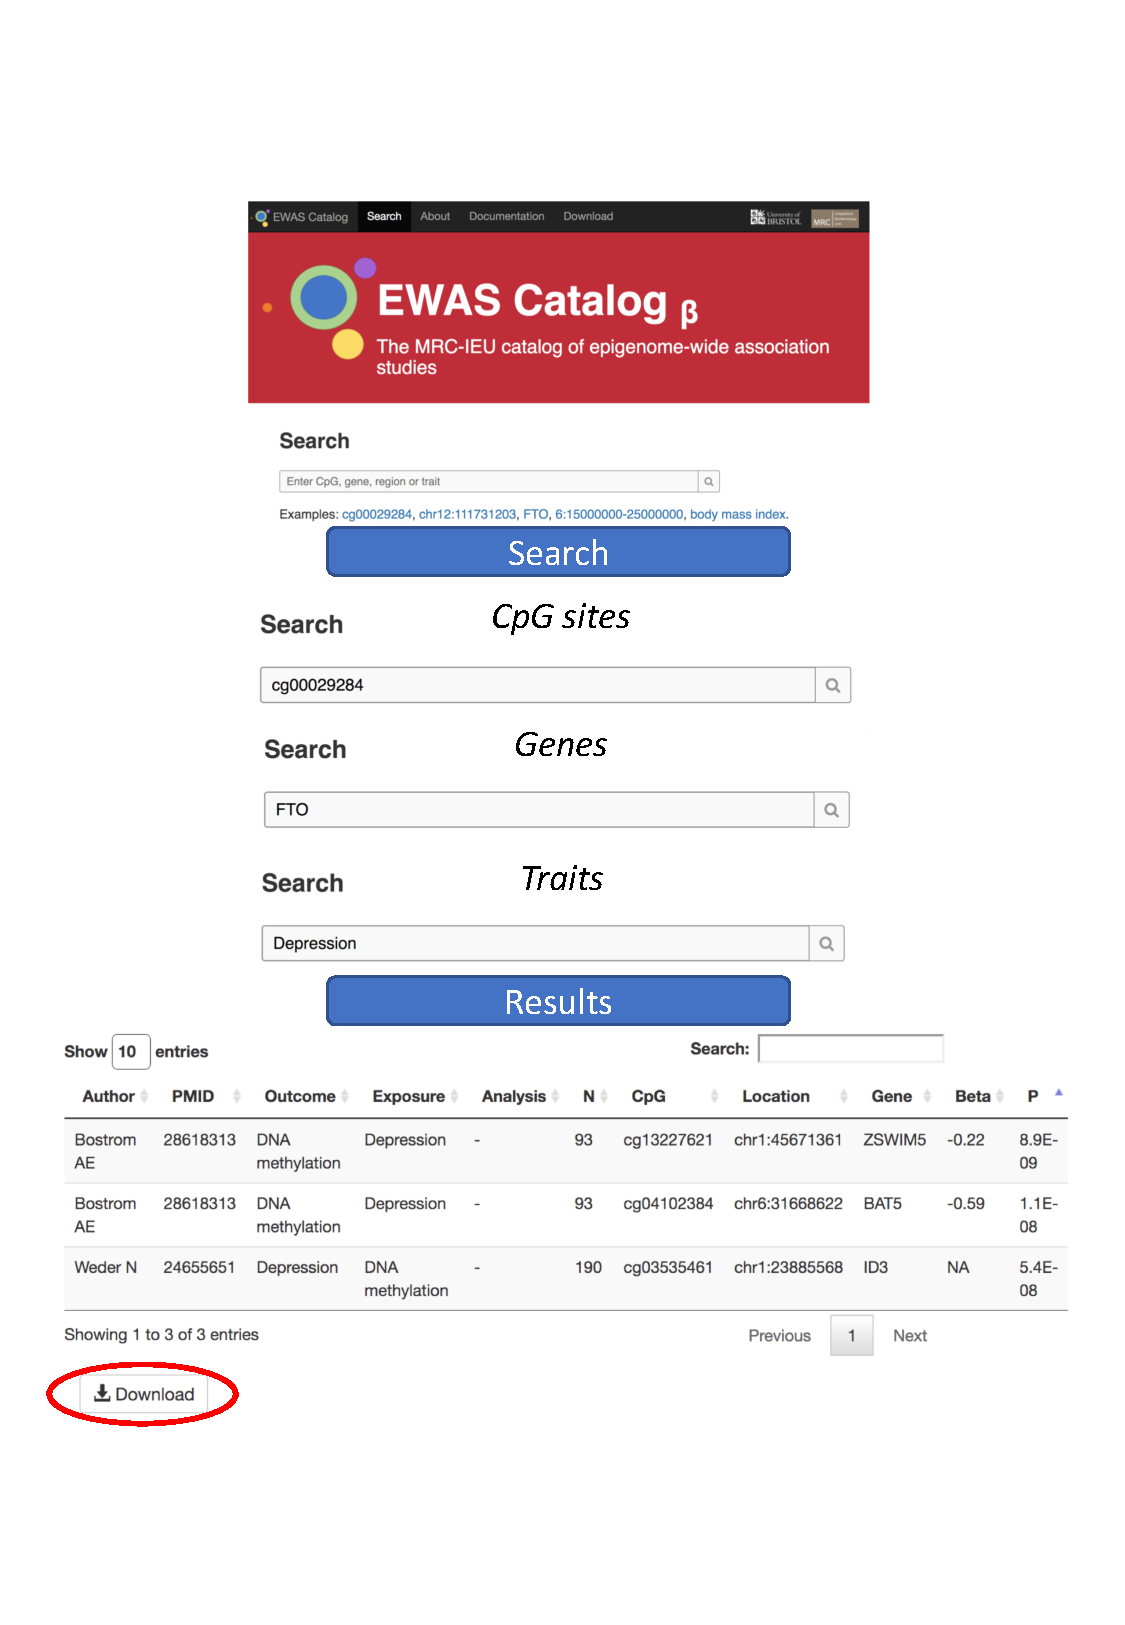
\includegraphics[width=1\linewidth]{/Users/tb13101/Desktop/projects/Main_project/thesis/index/figure/03-ewas_catalog/using_the_catalog} 

}

\caption{Using the EWAS catalog. 
At the top of the figures is the home page URL, ewascatalog.org. 
Below that are examples of three types of searches possible: 
1. CpG sites, 2. genes and 3. traits. 
Finally, the results are displayed after searching the catalog for “Depression”. 
Circled in red is the download button, this button enables the user to download the results of their search as a tab-separated value file. 
This file will contain the information shown on the website as well as additional analysis information.}\label{fig:catalog-use}
\end{figure}
The R package, along with installation instructions and examples are available at \url{https://github.com/ewascatalog/ewascatalog-r/}. Once installed, the database can be queried directly in R using the ``ewascatalog()'' function similar to the website: simply supply the function with a CpG site, gene, genome position or trait and the function returns the same output as is downloadable from the website.

\hypertarget{discussion}{%
\section{Discussion}\label{discussion}}

In this chapter, a database of previously published EWAS and the full summary statistics of 418 newly performed EWAS within ALSPAC and GEO has been established. This is freely available for all researchers to use and provides a platform to explore what information has been gained from EWAS as well as a platform that can be used to pool all existing data to gain new insights into both the EWAS study itself and how DNA methylation associates with traits. Despite the fact The EWAS Atlas has similar aims to The EWAS Catalog, latter provides full summary statistics, extra information and a user-friendly platform to enable more downstream analyses.

The EWAS catalog team will continue to collate and upload newly published EWAS and further increase the number of full summary statistics on the website by performing additional EWAS on available datasets and by inviting EWAS authors to provide full summary statistics. Currently work is ongoing to include additional functionality to allow users to easily and systematically compare their EWAS findings to EWAS in the database. With this full summary data, it is possible to make greater strides into discovering the epigenetic architecture of traits.

Therefore, despite the fact no extra information about EWAS was presented in this chapter, a platform has been made that easily enables us to explore 1) what information has been gained from EWAS and 2) the relationship between DNA methylation and all traits. This will be explored in the next chapters.

\hypertarget{properties-of-ewas}{%
\chapter{Properties of EWAS}\label{properties-of-ewas}}

Here is a reference to Caroline's paper: (Relton \& Davey Smith, 2010)

\hypertarget{h2ewas-chapter}{%
\chapter{h2ewas}\label{h2ewas-chapter}}

\hypertarget{ewas-gwas-comp-chapter}{%
\chapter{EWAS-GWAS comparison}\label{ewas-gwas-comp-chapter}}

\hypertarget{dnam-lung-cancer-mr}{%
\chapter{DNAm-lung cancer MR}\label{dnam-lung-cancer-mr}}

\hypertarget{abstract-1}{%
\section{Abstract}\label{abstract-1}}

\hypertarget{background}{%
\subsection{Background}\label{background}}

DNA methylation changes in peripheral blood have recently been identified in relation to lung cancer risk. Some of these changes have been suggested to mediate part of the effect of smoking on lung cancer. However, limitations with conventional mediation analyses mean that the causal nature of these methylation changes has yet to be fully elucidated.

\hypertarget{methods-2}{%
\subsection{Methods}\label{methods-2}}

We first performed a meta-analysis of four epigenome-wide association studies (EWAS) of lung cancer (918 cases, 918 controls). Next, we conducted a two-sample Mendelian randomization analysis, using genetic instruments for methylation at CpG sites identified in the EWAS meta-analysis, and 29,863 cases and 55,586 controls from the TRICL-ILCCO lung cancer consortium, to appraise the possible causal role of methylation at these sites on lung cancer.

\hypertarget{results-1}{%
\subsection{Results}\label{results-1}}

16 CpG sites were identified from the EWAS meta-analysis (FDR \textless{} 0.05), 14 of which we could identify genetic instruments for. Mendelian randomization provided little evidence that DNA methylation in peripheral blood at the 14 CpG sites play a causal role in lung cancer development (FDR \textgreater{} 0.05), including for cg05575921-\emph{AHRR} where methylation is strongly associated with both smoke exposure and lung cancer risk.

\hypertarget{conclusions}{%
\subsection{Conclusions}\label{conclusions}}

The results contrast with previous observational and mediation analysis, which have made strong claims regarding the causal role of DNA methylation. Thus, previous suggestions of a mediating role of methylation at sites identified in peripheral blood, such as cg05575921-\emph{AHRR}, could be unfounded. However, this study does not preclude the possibility that differential DNA methylation at other sites is causally involved in lung cancer development, especially within lung tissue.

\hypertarget{introduction-2}{%
\section{Introduction}\label{introduction-2}}

Lung cancer is the most common cause of cancer-related death worldwide (Ferlay et al., 2013). Several DNA methylation changes have been recently identified in relation to lung cancer risk (Baglietto et al., 2017; Fasanelli et al., 2015; McCarthy et al., 2016). Given the plasticity of epigenetic markers, any DNA methylation changes that are causally linked to lung cancer are potentially appealing targets for intervention (Jones \& Baylin, 2002; Strathdee \& Brown, 2002). However, these epigenetic markers are sensitive to reverse causation, being affected by cancer processes (Jones \& Baylin, 2002), and are also prone to confounding, for example by socio-economic and lifestyle factors {[}Borghol et al. (2012); Elliott2014{]}.

One CpG site, cg05575921 within the aryl hydrocarbon receptor repressor (\emph{AHRR}) gene, has been consistently replicated in relation to both smoking (Joehanes et al., 2016) and lung cancer (Baglietto et al., 2017; Bojesen, Timpson, Relton, Smith, \& Nordestgaard, 2017; Fasanelli et al., 2015) and functional evidence suggests that this region could be causally involved in lung cancer (Zudaire et al., 2008). However, the observed association between methylation and lung cancer might simply reflect separate effects of smoking on lung cancer and DNA methylation, i.e.~the association may be a result of confounding (Richmond, Hemani, Tilling, Davey Smith, \& Relton, 2016), including residual confounding after adjustment for self-reported smoking behaviour (Fewell, Davey Smith, \& Sterne, 2007; Munafò et al., 2012). Furthermore, recent epigenome-wide association studies (EWAS) for lung cancer have revealed additional CpG sites which may be causally implicated in development of the disease (Baglietto et al., 2017; Fasanelli et al., 2015).

Mendelian randomization (MR) uses genetic variants associated with modifiable factors as instruments to infer causality between the modifiable factor and outcome, overcoming most unmeasured or residual confounding and reverse causation (Davey Smith \& Ebrahim, 2003; Davey Smith \& Hemani, 2014). In order to infer causality, three core assumptions of MR should be met: 1) The instrument is associated with the exposure, 2) The instrument is not associated with any confounders, 3) The instrument is associated with the outcome only through the exposure. MR may be adapted to the setting of DNA methylation (Relton \& Davey Smith, 2012; Relton et al., 2015; Richardson et al., 2017) with the use of single nucleotide polymorphisms (SNPs) that correlate with methylation of CpG sites, known as methylation quantitative trait loci (mQTLs) (Gaunt et al., 2016).

In this study, we performed a meta-analysis of four lung cancer EWAS (918 case-control pairs) from prospective cohort studies to identify CpG sites associated with lung cancer risk and applied MR to investigate whether the observed DNA methylation changes at these sites are causally linked to lung cancer.

In this chapter, Dr Rebecca Richmond performed analysis in the CCHS cohort (see section \protect\hyperlink{potential-causal-effect-of-ahrr-methylation-on-lung-cancer-risk-one-sample-mr}{Potential causal effect of AHRR methylation on lung cancer risk: one sample MR} of the results) and contributed to writing the introduction and discussion. I completed all the analysis and wrote each section except the methods and results sections for which I did not complete the analysis.

\hypertarget{methods-3}{%
\section{Methods}\label{methods-3}}

\hypertarget{ewas-study-details}{%
\subsection{EWAS study details}\label{ewas-study-details}}

A meta-analysis of four lung cancer case-control EWAS was conducted to identify DNA methlyation sites associated with lung cancer. DNA methylation in each EWAS was assessed using the Illumina Infinium® HumanMethylation450 BeadChip. All EWAS are nested within prospective cohorts that measured DNA methylation in peripheral blood samples before diagnosis: EPIC-Italy (185 case-control pairs), Melbourne Collaborative Cohort Study (MCCS) (367 case-control pairs), Norwegian Women and Cancer (NOWAC) (132 case-control pairs) and the Northern Sweden Health and Disease Study (NSHDS) (234 case-control pairs). Study populations, laboratory methods, data pre-processing and quality control methods have been described in detail elsewhere (Baglietto et al., 2017) 3 and are outlined below.

At the various laboratory sites, samples were distributed into 96-well plates and processed in chips of 12 arrays (8 chips per plate) with case-control pairs arranged randomly on the same chip. Methylation data were pre-processed and normalized in each study, and probe filtering was performed as previously described (Baglietto et al., 2017), leaving 465,886 CpGs suitable for the analysis in EPIC-Italy, 485,330 CpGs in MCCS, 450,890 CpGs in NOWAC and 482,867 CpGs in NSHDS.

\hypertarget{european-prospective-investigation-into-cancer-and-nutrition-italy-epic-italy}{%
\subsubsection{European Prospective Investigation into Cancer and Nutrition-Italy (EPIC-Italy)}\label{european-prospective-investigation-into-cancer-and-nutrition-italy-epic-italy}}

EPIC-Italy includes 47,749 volunteers (32,579 women) aged 35--70 years at the time of recruitment (1992--1998). Anthropometric measurements and lifestyle variables including detailed information on smoking history were collected at recruitment through standardized questionnaires, together with a blood sample. Within EPIC-Italy we conducted a nested case-control study utilizing incident cases diagnosed within follow-up and healthy controls individually matched to cases by gender, date of birth (±5 years), date of inclusion in the study and study centre. Analysis was performed for 185 incident cases diagnosed within follow-up and matched controls. Laboratory procedures were carried out at the Human Genetics Foundation (Turin, Italy) and DNA extracted from buffy coats as previously described (Baglietto et al., 2017). All participants signed an informed consent form, and the ethical review boards of the International Agency for Research on Cancer and of each local participating centre approved the study protocol.

\hypertarget{melbourne-collaborative-cohort-study-mccs}{%
\subsubsection{Melbourne Collaborative Cohort Study (MCCS)}\label{melbourne-collaborative-cohort-study-mccs}}

The MCCS is a prospective cohort study of 41,514 volunteers (24,469 women) aged between 27 and 76 years at baseline (1990-1994). At baseline attendance, participants completed questionnaires that measured demographic characteristics and lifestyle factors. Height and weight were directly measured, and a blood sample was collected and stored. Incident cases of lung cancer were identified through linkage with the State and National Cancer Registries during follow-up up to the end of 2011. The MCCS sample included 367 cases and 367 matched controls selected from MCCS participants who were lung cancer free at the age of diagnosis of the matching case (density sampling). Matching variables included gender, date of blood collection (within 6 months), date of birth (within 1 year), country of birth (Australia and UK versus Southern Europe), type of biospecimen (lymphocyte, buffy coat and dried blood spot) and smoking status (never smokers; short-term former smokers: quitting smoking less than 10 years before blood draw; long-term former smokers: quitting smoking 10 years or more before blood draw; current light smokers: less than 15 cigarettes per day at blood draw; and current heavy smokers: 15 cigarettes or more at blood draw). For the MCCS, laboratory procedures were carried out at the Genetic Epidemiology Laboratory, the University of Melbourne according to manufacturers' protocols. DNA extraction from lymphocytes and buffy coats was performed as previously described (Baglietto et al., 2017). The Cancer Council Victoria's Human Research Ethics Committee approved the study protocol. Subjects gave written consent to participate and for the investigators to obtain access to their medical records.

\hypertarget{norwegian-women-and-cancer-nowac}{%
\subsubsection{Norwegian Women and Cancer (NOWAC)}\label{norwegian-women-and-cancer-nowac}}

The biobank of the NOWAC cohort was established in the years 2003-2006. Those who filled in an eight-page questionnaire and accepted the invitation to donate blood were sent blood drawing equipment together with a two-page epidemiological questionnaire. Around 50 000 women returned two tubes of blood to the Institute of Community Medicine at UiT The Arctic University of Norway and data linkage to the National Cancer Registry of Norway was performed. During follow-up to the end of 2011, 132 eligible cases of lung cancer were identified and were used for the EWAS. For each case, one control with an available blood sample was selected and matched on time since blood sampling and year of birth in order to control for effects of storage time and ageing. The cases and the controls were processed together for all laboratory procedures in order to reduce any batch effect. Laboratory procedures were carried out at the Human Genetics Foundation (Turin, Italy). DNA extraction from buffy coats was performed as previously described (Baglietto et al., 2017). All participants gave informed consent. The study was approved by the Regional Committee for Medical and Health Research Ethics in North Norway. Data storage and linkage was approved by the Norwegian Data Inspectorate.

\hypertarget{northern-sweden-health-and-disease-study-nshds}{%
\subsubsection{Northern Sweden Health and Disease Study (NSHDS)}\label{northern-sweden-health-and-disease-study-nshds}}

NSHDS is an ongoing prospective cohort and intervention study intended for health promotion of the population of Västerbotten County in northern Sweden. All residents were invited to participate by attending a health check-up at their local health care centre at 40, 50 and 60 years of age. At the health check-up, participants were asked to complete a self-administered questionnaire covering various factors such as education, smoking habits, physical activity and diet. In addition, height and weight were measured and participants were asked to donate a blood sample. Incident lung cancer cases were identified through linkage to the regional cancer registry. One control was chosen at random for each lung cancer case from appropriate risk sets consisting of all cohort members alive and free of cancer (except non-melanoma skin cancer) at the time of diagnosis of the index case. Matching criteria were the same as for the MCCS except there was no matching for type of biospecimens as DNA was extracted from whole blood for all samples. After quality control, a total of 234 incident lung cancer cases and 234 individually matched controls were available for this analysis. Laboratory procedures for NSHDS were carried out at two sites. DNA extraction from the buffy coat was conducted at Umeå University, Sweden, as previously described. Illumina Infinium HumanMethylation450 BeadChip analysis was conducted at the ALSPAC/IEU Laboratory at the University of Bristol. All study subjects provided written informed consent at time of the recruitment into the NSHDS.

\hypertarget{ewas-meta-analysis}{%
\subsection{EWAS Meta-analysis}\label{ewas-meta-analysis}}

To quantify the association between the methylation level at each CpG and the risk of lung cancer conditional logistic regression models were fitted for beta values of methylation (which ranges from 0 (no cytosines methylated) to 1 (all cytosines methylated)) on lung cancer status for the four studies. The cases and controls in each study were matched, details can be found above. Surrogate variables were computed in the four studies using the SVA R package (Leek et al., 2016) and the proportion of CD8+ and CD4+ T cells, B cells, monocytes, natural killer cells and granulocytes within whole blood were derived from DNA methylation (Houseman et al., 2012). The following EWAS models were included in the meta-analysis: Model 1 -- unadjusted; Model 2 -- adjusted for 10 surrogate variables (SVs); Model 3 -- adjusted for 10 SVs and derived cell proportions. EWAS stratified by smoking status was also conducted (never (N=304), former (N=648) and current smoking (N=857)). For Model 1 and Model 2, the case-control studies not matched on smoking status (EPIC-Italy and NOWAC) were adjusted for smoking.

An inverse-variance weighted fixed effects meta-analysis was performed of the EWAS (918 case-control pairs) using the \href{http://csg.sph.umich.edu/abecasis/metal/}{METAL software}. Direction of effect, effect estimates and the I\textsuperscript{2} statistic were used to assess heterogeneity across the studies in addition to effect estimates across smoking strata (never, former and current). All sites identified at a false discovery rate (FDR) \textless{} 0.05 in Model 2 and 3 were also present in the sites identified in Model 1. The effect size differences between models for all sites identified in Model 1 were assessed by a Kruskal-Wallis test and a post-hoc Dunn's test. There was little evidence for a difference (P \textgreater{} 0.1), so to maximize inclusion into the MR analyses we took forward the sites identified in the unadjusted model (Model 1).

\hypertarget{mendelian-randomization-1}{%
\subsection{Mendelian randomization}\label{mendelian-randomization-1}}

Two-sample MR was used to establish potential causal effect of differential methylation on lung cancer risk (Inoue \& Solon, 2010; Pierce \& Burgess, 2013).

\hypertarget{sample-1-accessible-resource-for-integrated-epigenomic-studies-aries}{%
\subsubsection{Sample 1: Accessible Resource for Integrated Epigenomic Studies (ARIES)}\label{sample-1-accessible-resource-for-integrated-epigenomic-studies-aries}}

In the first sample, mQTL-methylation effect estimates (\(\beta_{GP}\)) for each CpG site of interest were identified in an mQTL database from the Accessible Resource for Integrated Epigenomic Studies (ARIES) (\url{http://www.mqtldb.org}). Details on the methylation pre-processing, genotyping and quality control (QC) pipelines are outlined below.

\textbf{DNA methylation data}
Samples were drawn from the Avon Longitudinal Study of Parents and Children (2, 3). Blood from 1,018 mother--child pairs were selected for analysis as part of the Accessible Resource for Integrative Epigenomic Studies (ARIES, \url{http://www.ariesepigenomics.org.uk/}) (4). There are three timepoints in children and two in their mothers, the timepoints with mean ages (in brackets) in ARIES are as follows for children: birth, childhood (7.5), adolescence (17.1) and for mothers: during pregnancy (28.7), and at middle age (46.9). Following DNA extraction, samples were bisulphite converted using the Zymo EZ DNA Methylation\textsuperscript{TM} kit (Zymo, Irvine, CA, USA). Following conversion, genome-wide methylation was measured using the Illumina Infinium HumanMethylation450 (HM450) BeadChip. Methylation data were normalised in R with the watermelon package (5) using the Touleimat and Tost (6) algorithm to reduce the non-biological differences between probes. Methylation data in ARIES were rank-normalised to remove outliers, and then Matrix eQTL software (7) was used to perform preliminary association analysis of SNPs with all CpG sites in the Illumina Infinium HM450 array with the exception of those failing QC, and those reported to map to more than one location (n=19,834) or to contain a genetic variant at the CpG site (n=74,182) (8).

\textbf{Genetic data}
Children were genotyped using the Illumina HumanHap550 quad genome-wide SNP genotyping platform (Illumina Inc., San Diego, USA) by the Wellcome Trust Sanger Institute (WTSI, Cambridge, UK) and the Laboratory Corporation of America (LCA, Burlington, NC, USA). Individuals were excluded on the basis of incorrect gender assignment; abnormal heterozygosity (\textless0.320 or \textgreater0.345 for WTSI data; \textless0.310 or \textgreater0.330 for LCA data); high missingness (\textgreater3\%); cryptic relatedness (\textgreater10\% identity by descent) and non-European ancestry (detected by multidimensional scaling analysis). Following QC the final directly genotyped dataset contained 500,527 SNP loci.

Mothers were genotyped using the Illumina Human660W-quad genome-wide SNP genotyping platform (Illumina Inc., San Diego, USA) at the Centre National de Génotypage (CNG, Paris, France). Individuals were excluded based on non-European ancestry, missingness, relatedness, gender mismatches and heterozygosity. PLINK (v1.07) (9) was used to carry out quality control measures on an initial set of 10,015 subjects and 557,124 directly genotyped SNPs. Following QC the final directly genotyped dataset contained 526,688 SNP loci.

Imputation was performed to increase the SNP density for all genotyped mothers and children combined. Genotypes were phased together using ShapeIt, and then imputed against the 1000 genomes reference panel (phase 1 version 3, phased using ShapeIt version 2, December 2013, using all populations) using Impute (version 2.2.2). Genotypes were filtered to have Hardy-Weinberg equilibrium P \textgreater{} 5x10\textsuperscript{-7}, MAF \textgreater{} 1\% and imputation info score \textgreater{} 0.8. Best guess genotypes were used for subsequent analysis. The final imputed dataset used for the analyses presented here contained 8,074,398 loci.

Written informed consent has been obtained from all ALSPAC participants. Ethical approval for the study was obtained from the ALSPAC Ethics and Law Committee and Local Research Ethics Committees.
Please note that the study website contains details of all the data that is available through a fully searchable data dictionary: \url{http://www.bris.ac.uk/alspac/researchers/data-access/data-dictionary/}

\hypertarget{sample-2-transdisciplinary-research-in-cancer-of-the-lung-and-the-international-lung-cancer-consortium}{%
\subsection{Sample 2: Transdisciplinary Research in Cancer of the Lung and The International Lung Cancer Consortium}\label{sample-2-transdisciplinary-research-in-cancer-of-the-lung-and-the-international-lung-cancer-consortium}}

In the second sample, summary data was extracted from a GWAS meta-analysis of lung cancer risk conducted by the Transdisciplinary Research in Cancer of the Lung and The International Lung Cancer Consortium (TRICL-ILCCO) (29,863 cases, 55,586 controls) for individuals genotyped using the Illumina Infinium OncoArray-500K BeadChip (Illumina Inc.~San Diego, CA) and independent samples for which prior genotyping was performed (10). They were used to obtain mQTL-lung cancer estimates (\(\beta_{GD}\)) (McKay et al., 2017).

For each independent mQTL (r\textsuperscript{2} \textless{} 0.01), we calculated the log odds ratio (OR) per SD unit increase in methylation by the formula \(\frac{\beta_{GD}} {\beta_{GP}}\) (Wald ratio). Standard errors were approximated by the delta method (Thomas, Lawlor, \& Thompson, 2007). Where multiple independent mQTLs were available for one CpG site, these were combined in a fixed effects meta-analysis after weighting each ratio estimate by the inverse variance of their associations with the outcome. Heterogeneity in Wald ratios across mQTLs was estimated using Cochran's Q test, which can be used to indicate horizontal pleiotropy (Bowden, Smith, \& Burgess, 2015). Differences between the observational and MR estimates were assessed using a Z-test for difference.

If there was evidence for an mQTL-CpG site association in ARIES in at least one time-point, it was assessed whether the mQTL replicated across time points in ARIES (FDR \textless{} 0.05, same direction of effect). Further, this association was re-analysed using linear regression of methylation on each genotyped SNP available in an independent cohort (NSHDS), using rvtests (Zhan, Hu, Li, Abecasis, \& Liu, 2016). The same NSHDS samples on which DNA methylation was measured were genotyped using the Illumina Infinium OncoArray-500k BeadChip (Illumina Inc.~San Diego, CA) and quality control parameters were applied under the recently published TRICL-ILCCO GWAS study on lung cancer (10). Genetic imputation was performed on these samples using the Haplotype Reference Consortium (HRC) Panel (release 1) (11) through the Michigan Imputation Server (12). Replicated mQTLs were included where possible to reduce the effect of winner's curse using effect estimates from ARIES. We assessed the instrument strength of the mQTLs by investigating the variance explained in methylation by each mQTL (r\textsuperscript{2}) as well as the F-statistic in ARIES \textbf{Supplementary Table 1}. The power to detect the observational effect estimates in the two-sample MR analysis was assessed a priori, based on an alpha of 0.05, sample size of 29,863 cases and 55,586 controls (from TRICL-ILCCO) and calculated variance explained (r\textsuperscript{2}).

MR analyses were also performed to investigate the impact of methylation on lung cancer subtypes in TRICL-ILCCO: adenocarcinoma (11,245 cases, 54,619 controls), small cell carcinoma (2791 cases, 20,580 controls), and squamous cell carcinoma (7704 cases, 54,763 controls). We also assessed the association in never smokers (2303 cases, 6995 controls) and ever smokers (23,848 cases, 16,605 controls) (McKay et al., 2017) 25. Differences between the smoking subgroups were assessed using a Z-test for difference.

We next investigated the extent to which the mQTLs at cancer-related CpGs were associated with four smoking behaviour traits which could confound the methylation-lung cancer association: number of cigarettes per day, smoking cessation rate, smoking initiation and age of smoking initiation using GWAS data from the Tobacco and Genetics (TAG) consortium (N=74,053) (Furberg et al., 2010) 29.

\hypertarget{supplementary-analyses}{%
\subsection{Supplementary analyses}\label{supplementary-analyses}}

\hypertarget{assessing-the-potential-causal-effect-of-ahrr-methylation-one-sample-mr}{%
\subsubsection{\texorpdfstring{Assessing the potential causal effect of \emph{AHRR} methylation: one sample MR}{Assessing the potential causal effect of AHRR methylation: one sample MR}}\label{assessing-the-potential-causal-effect-of-ahrr-methylation-one-sample-mr}}

Given previous findings implicating methylation at \emph{AHRR} in relation to lung cancer (Baglietto et al., 2017; Fasanelli et al., 2015) 2, 3, we performed a one-sample MR analysis (Haycock et al., 2016) 30 of \emph{AHRR} methylation on lung cancer incidence using individual-level data from the Copenhagen City Heart Study (CCHS) (357 incident cases, 8401 remaining free of lung cancer). Copenhagen City Heart Study is a prospective study of the general population (13). Copenhagen residents were invited to complete a questionnaire and undergo a physical examination and are followed through a unique person identifier in the Danish health registries. All participants gave written informed consent, and a Danish ethics committee approved the study (KF100.2039/91).

\textbf{Phenotypic data}
Participants were asked whether they smoked at the day of attendance or previously. If they answered affirmative to either of these questions, they were asked about their current and former smoking behaviour, including age of smoking initiation, age of smoking cessation, and number of daily consumed cigarettes, cheroots, cigars, and weekly grams of pipe tobacco. Based on these answers, participants were categorized as never, former, and current smokers. In addition, participants reported on alcohol consumption, occupational exposure to dust and/or welding fumes, exposure to passive smoking, education, and familial cases of lung cancer. The answers were reviewed together with an examiner at the day of attendance. Body mass index was calculated as measured weight in kilograms divided by measured height (in meters) squared.

\textbf{Methylation data}
At the physical examination, blood samples were drawn for DNA from which AHRR methylation extent was measured (14). The AHRR cg05575921 methylation extent was measured in duplicate samples of bisulphite treated DNA from peripheral blood from 9,234 individuals. We used a Taqman assay developed in our own laboratory, and included standard curves, as well as internal controls in each 384-well plate. Coefficients of variation at the methylation level of 71\% varied from 5.0 to 6.7\%. Laboratory technicians were blinded to smoking and disease status of the individuals. Results were validated with pyrosequencing on a subset of samples.

\textbf{Genetic data}
Genotypes from the iCOGs array (15) and prospective data on lung cancer incidence were also available for these participants. Of the 9234 individuals, genotype data from iCOGS on 8778 were available. In short, DNA isolated from leukocytes was genotyped with a custom Illumina iSelect genotyping array, designed to test genetic variants related to breast, ovary and prostate cancer, comprising roughly 211,000 SNPs after rigorous quality control (15).

\textbf{Lung cancer data}
For lung cancer (ICD7, codes 1624 or 4624 until 1977, and ICD10, code C34 from 1978 and onwards), the date of first diagnosis was taken from the national Danish Cancer Registry from 1943 to December 2012.

\textbf{Identification of mQTLs for CCHS one-sample MR}
mQTLs located within 1Mb of cg05575921 \emph{AHRR} were identified in ARIES (FDR\textless0.05). Of those mQTLs which replicated within the CCHS, we performed an LD pruning step using a less stringent r\textsuperscript{2} threshold of 0.2 and generated an unweighted allele score, calculated by coding and then summing the alleles to reflect the average number of methylation-increasing alleles carried by an individual. Associations between the allele score and several potential confounding factors (sex, alcohol consumption, smoking status, occupational exposure to dust and/or welding fumes, passive smoking) were investigated. Then MR analyses were performed using two-stage Cox regression, with adjustment for age and sex, and further stratified by smoking status.

\hypertarget{tumour-and-adjacent-normal-methylation-patterns}{%
\subsubsection{Tumour and adjacent normal methylation patterns}\label{tumour-and-adjacent-normal-methylation-patterns}}

DNA methylation data from lung cancer tissue and matched normal adjacent tissue (N=40 squamous cell carcinoma and N=29 adenocarcinoma), profiled as part of The Cancer Genome Atlas (TCGA), were used to assess tissue-specific DNA methylation changes across sites identified in the meta-analysis of EWAS, as outlined previously (Teschendorff et al., 2015) 31.

\hypertarget{mqtl-association-with-gene-expression}{%
\subsubsection{mQTL association with gene expression}\label{mqtl-association-with-gene-expression}}

For the genes annotated to CpG sites identified in the lung cancer EWAS, we examined gene expression in whole blood and lung tissue using data from the gene-tissue expression (GTEx) consortium (GTEx Consortium, 2013) 32.

Analyses were conducted in Stata (version 14) and R (version 3.2.2). For the two-sample MR analysis we used the MR-Base R package TwoSampleMR (Hemani et al., 2016) 33. An adjusted P value that limited the FDR was calculated using the Benjamini-Hochberg method (Benjamini \& Hochberg, 1995) 34. All statistical tests were two-sided.

\hypertarget{results-2}{%
\section{Results}\label{results-2}}

A flowchart representing our study design along with a summary of our results at each step is displayed in Figure 1.

(Figure 1 here)

\hypertarget{ewas-meta-analysis-1}{%
\subsection{EWAS meta-analysis}\label{ewas-meta-analysis-1}}

The basic meta-analysis adjusted for study-specific covariates identified 16 CpG sites which were hypomethylated in relation to lung cancer (FDR\textless0.05, Model 1, Figure 2). Adjusting for 10 surrogate variables (Model 2) and derived cell counts (Model 3) gave similar results (Table 1). The direction of effect at the 16 sites did not vary between studies (median I2=38.6) (Supplementary Table 2), but there was evidence for heterogeneity of effect estimates at some sites when stratifying individuals by smoking status (Table 1).

(Figure 2 here)

(Table 1 here)

\hypertarget{mendelian-randomization-2}{%
\subsection{Mendelian randomization}\label{mendelian-randomization-2}}

We identified 15 independent mQTLs (r2\textless0.01) associated with methylation at 14 of 16 CpGs. Ten mQTLs replicated at FDR\textless0.05 in NSHDS (Supplementary Table 3). MR power analyses indicated \textgreater99\% power to detect ORs for lung cancer of the same magnitude as those in the meta-analysis of EWAS.

There was little evidence for an effect of methylation at these 14 sites on lung cancer (FDR\textgreater0.05, Supplementary Table 4). For nine of 14 CpG sites the point estimates from the MR analysis were in the same direction as in the EWAS, but of a much smaller magnitude (Z-test for difference, P\textless0.001) (Figure 3).

For 9 of out the 16 mQTL-CpG associations, there was strong replication across time points (Supplementary Table 5) and 10 out of 16 mQTL-CpG associations replicated at FDR\textless0.05 in an independent adult cohort (NSHDS). Using mQTL effect estimates from NSHDS for the 10 CpG sites that replicated (FDR\textless0.05), findings were consistent with limited evidence for a causal effect of peripheral blood-derived DNA methylation on lung cancer (Supplementary Figure 1).

(Figure 3 here)

There was little evidence of different effect estimates between ever and never smokers at individual CpG sites (Supplementary Figure 2, Z-test for difference, P\textgreater0.5). There was some evidence for a possible effect of methylation at cg21566642-ALPPL2 and cg23771366-PRSS23 on squamous cell lung cancer (OR=0.85 {[}95\% confidence interval (CI)=0.75,0.97{]} and 0.91 {[}95\% CI=0.84,1.00{]} per SD {[}14.4\% and 5.8\%{]} increase, respectively) as well as methylation at cg23387569-AGAP2, cg16823042-AGAP2, and cg01901332-ARRB1 on lung adenocarcinoma (OR=0.86 {[}95\% CI=0.77,0.96{]}, 0.84 {[}95\% CI=0.74,0.95{]}, and 0.89 {[}95\% CI=0.80,1.00{]} per SD {[}9.47\%, 8.35\%, and 8.91\%{]} increase, respectively). However, none of the results withstood multiple testing correction (FDR\textless0.05) (Supplementary Figure 3). For those CpGs where multiple mQTLs were used as instruments (cg05575921-AHRR and cg01901332-ARRB1), there was limited evidence for heterogeneity in MR effect estimates (Q-test, P\textgreater0.05, Supplementary Table 6).

Single mQTLs for cg05575921-AHRR, cg27241845-ALPPL2, and cg26963277-KCNQ1 showed some evidence of association with smoking cessation (former vs.~current smokers), although these associations were not below the FDR\textless0.05 threshold (Supplementary Figure 4).

\hypertarget{potential-causal-effect-of-ahrr-methylation-on-lung-cancer-risk-one-sample-mr}{%
\subsubsection{Potential causal effect of AHRR methylation on lung cancer risk: one sample MR}\label{potential-causal-effect-of-ahrr-methylation-on-lung-cancer-risk-one-sample-mr}}

In the CCHS, a per (average methylation-increasing) allele change in a four-mQTL allele score was associated with a 0.73\% {[}95\% CI=0.56,0.90{]} increase in methylation (P\textless1 x 10-10) and explained 0.8\% of the variance in cg05575921-AHRR methylation (F-statistic=74.2). Confounding factors were not strongly associated with the genotypes in this cohort (P\textgreater=0.11) (Supplementary Table 7). Results provided some evidence for an effect of cg05575921 methylation on total lung cancer risk (HR=0.30 {[}95\% CI=0.10,1.00{]} per SD (9.2\%) increase) (Supplementary Table 8). The effect estimate did not change substantively when stratified by smoking status (Supplementary Table 8).

Given contrasting findings with the main MR analysis, where cg05575921-AHRR methylation was not causally implicated in lung cancer, and the lower power in the one-sample analysis to detect an effect of equivalent size to the observational results (power = 19\% at alpha = 0.05), we performed further two-sample MR based on the four mQTLs using data from both CCHS (sample one) and the TRICL-ILCCO consortium (sample two). Results showed no strong evidence for a causal effect of DNA methylation on total lung cancer risk (OR=1.00 {[}95\% CI=0.83,1.10{]} per SD increase) (Supplementary Figure 5). There was also limited evidence for an effect of cg05575921-AHRR methylation when stratified by cancer subtype and smoking status (Supplementary Figure 5) and no strong evidence for heterogeneity of the mQTL effects (Supplementary Table 9). Conclusions were consistent when MR-Egger (27) was applied (Supplementary Figure 5) and when accounting for correlation structure between the mQTLs (Supplementary Table 9).

\hypertarget{tumour-and-adjacent-normal-lung-tissue-methylation-patterns}{%
\subsection{Tumour and adjacent normal lung tissue methylation patterns}\label{tumour-and-adjacent-normal-lung-tissue-methylation-patterns}}

For cg05575921-AHRR, there was no strong evidence for differential methylation between adenocarcinoma tissue and adjacent healthy tissue (P=0.963), and weak evidence for hypermethylation in squamous cell carcinoma tissue (P=0.035) (Figure 4, Supplementary Table 10). For the other CpG sites there was evidence for a difference in DNA methylation between tumour and healthy adjacent tissue at several sites in both adenocarcinoma and squamous cell carcinoma, with consistent differences for CpG sites in ALPPL2 (cg2156642, cg05951221 and cg01940273), as well as cg23771366-PRSS23, cg26963277-KCNQ1, cg09935388-GFI1, cg0101332-ARRB1, cg08709672-AVPR1B and cg25305703-CASC21. However, hypermethylation in tumour tissue was found for the majority of these sites, which is opposite to what was observed in the EWAS analysis.

(Figure 4 here)

\hypertarget{gene-expression-associated-with-mqtls-in-blood-and-lung-tissue}{%
\subsection{Gene expression associated with mQTLs in blood and lung tissue}\label{gene-expression-associated-with-mqtls-in-blood-and-lung-tissue}}

Of the 10 genes annotated to the 14 CpG sites, eight genes were expressed sufficiently to be detected in lung (AVPR1B and CASC21 were not) and seven in blood (AVPR1B, CASC21 and ALPPL2 were not). Of these, gene expression of ARRB1 could not be investigated as the mQTLs in that region were not present in the GTEx data. rs3748971 and rs878481, mQTLs for cg21566642 and cg05951221 respectively, were associated with increased expression of ALPPL2 (P=0.002 and P=0.0001). No other mQTLs were associated with expression of the annotated gene at a Bonferroni corrected P value threshold (P\textless0.05/19=0.0026) (Supplementary Table 11).

\hypertarget{discussion-1}{%
\section{Discussion}\label{discussion-1}}

In this study, we identified 16 CpG sites associated with lung cancer, of which 14 have been previously identified in relation to smoke exposure (Joehanes et al., 2016) 9 and six were highlighted in a previous study as being associated with lung cancer (Baglietto et al., 2017) 3. This previous study used the same data from the four cohorts investigated here, but in a discovery and replication, rather than meta-analysis framework. Overall, using MR we found limited evidence supporting a potential causal effect of methylation at the CpG sites identified in peripheral blood on lung cancer. These findings are in contrast to previous analyses suggesting that methylation at two CpG sites investigated (in AHRR and F2RL3) mediated \textgreater{} 30\% of the effect of smoking on lung cancer risk (Fasanelli et al., 2015) 2. This previous study used methods which are sensitive to residual confounding and measurement error that may have biased results {[}Richmond et al. (2016); Hemani2017{]} 12, 35. These limitations are largely overcome using MR (Richmond et al., 2016) 12. While there was some evidence for an effect of methylation at some of the other CpG sites on risk of subtypes of lung cancer, these effects were not robust to multiple testing correction and were not validated in the analysis of tumour and adjacent normal lung tissue methylation nor in gene expression analysis.

A major strength of the study was the use of two-sample MR to integrate an extensive epigenetic resource and summary data from a large lung cancer GWAS to appraise causality of observational associations with \textgreater99\% power. Evidence against the observational findings were also acquired through tissue-specific DNA methylation and gene expression analyses.

Limitations include potential ``winner's curse'' which may bias causal estimates in a two-sample MR analysis towards the null if the discovery sample for identifying genetic instruments is used as the first sample, as was done for our main MR analysis using data from ARIES (Burgess \& Thompson, 2011) 36. However, findings were similar when using replicated mQTLs in NSHDS, indicating the potential impact of this bias was minimal (Supplementary Figure 1). Another limitation relates to the potential issue of consistency and validity of the instruments across the two samples. For a minority of the mQTL-CpG associations (4 out of 16), there was limited replication across time points and in particular, 6 mQTLs were not strongly associated with DNA methylation in adults. Further, our primary data used for the first sample in the two-sample MR was ARIES, which contains no male adults. If the mQTLs identified vary by sex and time, then this could bias our results. However, our replication cohort NSHDS contains adult males. Therefore, the 10 mQTLs that replicated in NSHDS are unlikely to be biased by the sex discordance. Also, we replicated the findings for cg05575921 \emph{AHRR} in CCHS, which contains both adult males and females, in a two-sample MR analysis, suggesting these results are also not influenced by sex discordance. Caution is therefore warranted when interpreting the null results for the two-sample MR estimates for the CpG sites for which mQTLs were not repliacted, which could be the result of weak-instrument bias.

The lack of independent mQTLs for each CpG site did not allow us to properly appraise horizontal pleiotropy in our MR analyses. Where possible we only included cis-acting mQTLs to minimise pleiotropy and investigated heterogeneity where there were multiple independent mQTLs. Three mQTLs were nominally associated with smoking phenotypes, but not to the extent that this would bias our MR results substantially. Some of the mQTLs used influence multiple CpGs in the same region, suggesting genomic control of methylation at a regional rather than single CpG level. This was untested, but methods to detect differentially methylated regions (DMRs) and identify genetic variants which proxy for them may be fruitful in probing the effect of methylation across gene regions.

A further limitation relates to the inconsistency in effect estimates between the one- and two-sample MR analysis to appraise the causal role of AHRR methylation. While findings in CCHS were supportive of a causal effect of AHRR methylation on lung cancer (HR=0.30 {[}95\% CI=0.10,1.00{]} per SD), in two-sample MR this site was not causally implicated (OR=1.00 {[}95\% CI=0.83,1.10{]} per SD increase). We verified that this was not due to differences in the genetic instruments used, nor due to issues of weak instrument bias. Given the CCHS one-sample MR had little power (19\% at alpha = 0.05) to detect a causal effect with a size equivalent to that of the observational analysis, we have more confidence in the results from the two-sample approach.

Peripheral blood may not be the ideal tissue to assess the association between DNA methylation and lung cancer. While a high degree of concordance in mQTLs has been observed across lung tissue, skin and peripheral blood DNA (Shi et al., 2014) 37, we were unable to directly evaluate this here. A possible explanation for a lack of causal effect at AHRR is due to the limitation of tissue specificity as we found that the mQTLs used to instrument cg05575921 were not strongly related to expression of AHRR in lung tissue. However, findings from MR analysis were corroborated by the lack of evidence for differential methylation at AHRR between lung adenocarcinoma tissue and adjacent healthy tissue, and weak evidence for hypermethylation (opposite to the expected direction) in squamous cell lung cancer tissue. This result may be interesting in itself as smoking is hypothesized to influence squamous cell carcinoma more than adenocarcinoma. However, the result conflicts with that found in the MR analysis. Furthermore, another study investigating tumorous lung tissue (N=511) found only weak evidence for an association between smoking and cg05575921 AHRR methylation, that did not survive multiple testing correction (P=0.02) (Freeman, Chu, Hsu, \& Huang, 2016) 38. However, our results do not fully exclude AHRR from involvement in the disease process. AHRR and AHR form a regulatory feedback loop, which means that the actual effect of differential methylation or differential expression of AHR/AHRR on pathway activity is complex (Chen et al., 2017) 39. In addition, some of the CpG sites identified in the EWAS were found to be differentially methylated in the tumour and adjacent normal lung tissue comparison. While this could represent a false negative result of the MR analysis, it is of interest that differential methylation in the tissue comparison analysis was typically in the opposite direction to that observed in the EWAS. Furthermore, while this method can be used to minimize confounding, it does not fully eliminate the possibility of bias due to reverse causation (whereby cancer induces changes in DNA methylation) or intra-individual confounding e.g.~by gene expression. Therefore, it doesn't give conclusive evidence that DNA methylation changes at these sites are not relevant to the development of lung cancer.

While DNA methylation in peripheral blood may be predictive of lung cancer risk, according to the present analysis it is unlikely to play a causal role in lung carcinogenesis at the CpG sites investigated. Findings from this study issue caution over the use of traditional mediation analyses to implicate intermediate biomarkers (such as DNA methylation) in pathways linking an exposure with disease, given the potential for residual confounding in this context (Richmond et al., 2016) 12. However, the findings of this study do not preclude the possibility that other DNA methylation changes are causally related to lung cancer (or other smoking-associated disease) (Gao, Zhang, Breitling, \& Brenner, 2016) 40.

\hypertarget{conclusion}{%
\chapter*{Conclusion}\label{conclusion}}
\addcontentsline{toc}{chapter}{Conclusion}

If we don't want Conclusion to have a chapter number next to it, we can add the \texttt{\{-\}} attribute.

\textbf{More info}

And here's some other random info: the first paragraph after a chapter title or section head \emph{shouldn't be} indented, because indents are to tell the reader that you're starting a new paragraph. Since that's obvious after a chapter or section title, proper typesetting doesn't add an indent there.

\appendix

\hypertarget{the-first-appendix}{%
\chapter{The First Appendix}\label{the-first-appendix}}

This first appendix includes all of the R chunks of code that were hidden throughout the document (using the \texttt{include\ =\ FALSE} chunk tag) to help with readibility and/or setup.

\textbf{In the main Rmd file}

\textbf{In Chapter \ref{ref-labels}:}

\hypertarget{the-second-appendix-for-fun}{%
\chapter{The Second Appendix, for Fun}\label{the-second-appendix-for-fun}}

\backmatter

\hypertarget{references}{%
\chapter*{References}\label{references}}
\addcontentsline{toc}{chapter}{References}

\markboth{References}{References}

\noindent

\setlength{\parindent}{-0.20in}
\setlength{\leftskip}{0.20in}
\setlength{\parskip}{8pt}

\hypertarget{refs}{}
\begin{cslreferences}
\leavevmode\hypertarget{ref-Baglietto2017}{}%
Baglietto, L., Ponzi, E., Haycock, P., Hodge, A., Bianca Assumma, M., Jung, C. H., \ldots{} Severi, G. (2017). DNA methylation changes measured in pre-diagnostic peripheral blood samples are associated with smoking and lung cancer risk. \emph{International Journal of Cancer}, \emph{140}(1), 50--61. \url{http://doi.org/10.1002/ijc.30431}

\leavevmode\hypertarget{ref-Banos2018}{}%
Banos, D. T., McCartney, D. L., Battram, T., Hemani, G., Walker, R. M., Morris, S. W., \ldots{} Robinson, M. R. (2018). Bayesian reassessment of the epigenetic architecture of complex traits. \emph{bioRxiv}, 450288. \url{http://doi.org/10.1101/450288}

\leavevmode\hypertarget{ref-Benjamini1995}{}%
Benjamini, Y., \& Hochberg, Y. (1995). Controlling the False Discovery Rate: A Practical and Powerful Approach to Multiple Testing. \emph{Journal of the Royal Statistical Society: Series B (Methodological)}. \url{http://doi.org/10.1111/j.2517-6161.1995.tb02031.x}

\leavevmode\hypertarget{ref-Bojesen2017}{}%
Bojesen, S. E., Timpson, N., Relton, C., Smith, G. D., \& Nordestgaard, B. G. (2017). AHRR (cg05575921) hypomethylation marks smoking behaviour, morbidity and mortality. \emph{Thorax}, no pagination. \url{http://doi.org/10.1136/thoraxjnl-2016-208789}

\leavevmode\hypertarget{ref-Borghol2012}{}%
Borghol, N., Suderman, M., Mcardle, W., Racine, A., Hallett, M., Pembrey, M., \ldots{} Szyf, M. (2012). Associations with early-life socio-economic position in adult DNA methylation. \emph{International Journal of Epidemiology}. \url{http://doi.org/10.1093/ije/dyr147}

\leavevmode\hypertarget{ref-Bowden2015}{}%
Bowden, J., Smith, G. D., \& Burgess, S. (2015). Mendelian randomization with invalid instruments: Effect estimation and bias detection through Egger regression. \emph{International Journal of Epidemiology}, \emph{44}(2), 512--525. \url{http://doi.org/10.1093/ije/dyv080}

\leavevmode\hypertarget{ref-Boyd2013}{}%
Boyd, A., Golding, J., Macleod, J., Lawlor, D. A., Fraser, A., Henderson, J., \ldots{} Smith, G. D. (2013). Cohort profile: The 'Children of the 90s'-The index offspring of the avon longitudinal study of parents and children. \emph{International Journal of Epidemiology}, \emph{42}(1), 111--127. \url{http://doi.org/10.1093/ije/dys064}

\leavevmode\hypertarget{ref-Buniello2019}{}%
Buniello, A., Macarthur, J. A. L., Cerezo, M., Harris, L. W., Hayhurst, J., Malangone, C., \ldots{} Parkinson, H. (2019). The NHGRI-EBI GWAS Catalog of published genome-wide association studies, targeted arrays and summary statistics 2019. \emph{Nucleic Acids Research}. \url{http://doi.org/10.1093/nar/gky1120}

\leavevmode\hypertarget{ref-Burgess2011}{}%
Burgess, S., \& Thompson, S. G. (2011). Avoiding bias from weak instruments in mendelian randomization studies. \emph{International Journal of Epidemiology}. \url{http://doi.org/10.1093/ije/dyr036}

\leavevmode\hypertarget{ref-Chen2017}{}%
Chen, J., Behnam, E., Huang, J., Moffatt, M. F., Schaid, D. J., Liang, L., \& Lin, X. (2017). Fast and robust adjustment of cell mixtures in epigenome-wide association studies with SmartSVA. \emph{BMC Genomics}. \url{http://doi.org/10.1186/s12864-017-3808-1}

\leavevmode\hypertarget{ref-DaveySmith2003}{}%
Davey Smith, G., \& Ebrahim, S. (2003). 'Mendelian randomization': Can genetic epidemiology contribute to understanding environmental determinants of disease? \url{http://doi.org/10.1093/ije/dyg070}

\leavevmode\hypertarget{ref-DaveySmith2014}{}%
Davey Smith, G., \& Hemani, G. (2014). Mendelian randomization: genetic anchors for causal inference in epidemiological studies. \emph{Human Molecular Genetics}, \emph{23}(R1), R89--98. \url{http://doi.org/10.1093/hmg/ddu328}

\leavevmode\hypertarget{ref-Fasanelli2015}{}%
Fasanelli, F., Baglietto, L., Ponzi, E., Guida, F., Campanella, G., Johansson, M., \ldots{} Vineis, P. (2015). Hypomethylation of smoking-related genes is associated with future lung cancer in four prospective cohorts. \emph{Nature Communications}, \emph{6}, 10192. \url{http://doi.org/10.1038/ncomms10192}

\leavevmode\hypertarget{ref-Ferlay2013}{}%
Ferlay, J., Soerjomataram, I., Ervik, M., Dikshit, R., Eser, S., Mathers, C., \ldots{} Bray, F. (2013). GLOBOCAN 2012 v1.0, Cancer Incidence and Mortality Worldwide: IARC CancerBase. No. 11 {[}Internet{]}., \emph{11}, http://globocan.iarc.f. \url{http://doi.org/10.1016/j.ucl.2013.01.011}

\leavevmode\hypertarget{ref-Fewell2007}{}%
Fewell, Z., Davey Smith, G., \& Sterne, J. A. C. (2007). The impact of residual and unmeasured confounding in epidemiologic studies: A simulation study. \emph{American Journal of Epidemiology}. \url{http://doi.org/10.1093/aje/kwm165}

\leavevmode\hypertarget{ref-Fraser2013}{}%
Fraser, A., Macdonald-wallis, C., Tilling, K., Boyd, A., Golding, J., Davey smith, G., \ldots{} Lawlor, D. A. (2013). Cohort profile: The avon longitudinal study of parents and children: ALSPAC mothers cohort. \emph{International Journal of Epidemiology}. \url{http://doi.org/10.1093/ije/dys066}

\leavevmode\hypertarget{ref-Freeman2016}{}%
Freeman, J. R., Chu, S., Hsu, T., \& Huang, Y.-t. (2016). Epigenome-wide association study of smoking and DNA methylation in non-small cell lung neoplasms. \emph{Oncotarget}, \emph{7}(43). \url{http://doi.org/10.18632/oncotarget.11831}

\leavevmode\hypertarget{ref-Furberg2010}{}%
Furberg, H., Kim, Y., Dackor, J., Boerwinkle, E., Franceschini, N., Ardissino, D., \ldots{} Sullivan, P. F. (2010). Genome-wide meta-analyses identify multiple loci associated with smoking behavior. \emph{Nature Genetics}. \url{http://doi.org/10.1038/ng.571}

\leavevmode\hypertarget{ref-Gao2016}{}%
Gao, X., Zhang, Y., Breitling, L. P., \& Brenner, H. (2016). Tobacco smoking and methylation of genes related to lung cancer development. \emph{Oncotarget}. \url{http://doi.org/10.18632/oncotarget.10007}

\leavevmode\hypertarget{ref-Gaunt2016}{}%
Gaunt, T. R., Shihab, H. A., Hemani, G., Min, J. L., Woodward, G., Lyttleton, O., \ldots{} Relton, C. L. (2016). Systematic identification of genetic influences on methylation across the human life course. \emph{Genome Biology}, \emph{17}(1), 61. \url{http://doi.org/10.1186/s13059-016-0926-z}

\leavevmode\hypertarget{ref-GTExConsortium2013}{}%
GTEx Consortium, T. G. (2013). The Genotype-Tissue Expression (GTEx) project. \emph{Nature Genetics}, \emph{45}(6), 580--5. \url{http://doi.org/10.1038/ng.2653}

\leavevmode\hypertarget{ref-Haycock2016}{}%
Haycock, P. C., Burgess, S., Wade, K. H., Bowden, J., Relton, C., \& Smith, G. D. (2016). Best (but oft-forgotten) practices: The design, analysis, and interpretation of Mendelian randomization studies. \emph{American Journal of Clinical Nutrition}. \url{http://doi.org/10.3945/ajcn.115.118216}

\leavevmode\hypertarget{ref-Hemani2016}{}%
Hemani, G., Zheng, J., Wade, K. H., Laurin, C., Elsworth, B., Burgess, S., \ldots{} Haycock, P. C. (2016). MR-Base: a platform for systematic causal inference across the phenome using billions of genetic associations. \emph{bioRxiv}. Retrieved from \url{http://biorxiv.org/content/early/2016/12/16/078972.abstract}

\leavevmode\hypertarget{ref-Horvath2013}{}%
Horvath, S. (2013). DNA methylation age of human tissues and cell types. \emph{Genome Biology}, \emph{14}(10), R115. \url{http://doi.org/10.1186/gb-2013-14-10-r115}

\leavevmode\hypertarget{ref-Houseman2012}{}%
Houseman, E. A., Accomando, W. P., Koestler, D. C., Christensen, B. C., Marsit, C. J., Nelson, H. H., \ldots{} Kelsey, K. T. (2012). DNA methylation arrays as surrogate measures of cell mixture distribution. \emph{BMC Bioinformatics}. \url{http://doi.org/10.1186/1471-2105-13-86}

\leavevmode\hypertarget{ref-Huang2015}{}%
Huang, W. Y., Hsu, S. D., Huang, H. Y., Sun, Y. M., Chou, C. H., Weng, S. L., \& Huang, H. D. (2015). MethHC: A database of DNA methylation and gene expression in human cancer. \emph{Nucleic Acids Research}. \url{http://doi.org/10.1093/nar/gku1151}

\leavevmode\hypertarget{ref-Inoue2010}{}%
Inoue, A., \& Solon, G. (2010). Two-Sample Instrumental variables estimators. \emph{The Review of Economics and Statistics}, \emph{92}(3), 557--561. \url{http://doi.org/10.1016/0304-4076(90)90061-W}

\leavevmode\hypertarget{ref-Joehanes2016}{}%
Joehanes, R., Just, A. C., Marioni, R. E., Pilling, L. C., Reynolds, L. M., Mandaviya, P. R., \ldots{} London, S. J. (2016). Epigenetic Signatures of Cigarette Smoking. \emph{Circulation: Cardiovascular Genetics}, \emph{9}(5), 436--447. \url{http://doi.org/10.1161/CIRCGENETICS.116.001506}

\leavevmode\hypertarget{ref-Jones2002}{}%
Jones, P. a, \& Baylin, S. B. (2002). The fundamental role of epigenetic events in cancer. \emph{Nature Reviews. Genetics}, \emph{3}(6), 415--28. \url{http://doi.org/10.1038/nrg816}

\leavevmode\hypertarget{ref-Leek2016}{}%
Leek, J. T., Johnson, W. E., Parker, H. S., Fertig, E. J., Jaffe, A. E., \& Storey, J. D. (2016). sva: Surrogate Variable Analysis.

\leavevmode\hypertarget{ref-Li2011}{}%
Li, H. (2011). Tabix: Fast retrieval of sequence features from generic TAB-delimited files. \emph{Bioinformatics}. \url{http://doi.org/10.1093/bioinformatics/btq671}

\leavevmode\hypertarget{ref-Li2019}{}%
Li, M., Zou, D., Li, Z., Gao, R., Sang, J., Zhang, Y., \ldots{} Zhang, Z. (2019). EWAS Atlas: A curated knowledgebase of epigenome-wide association studies. \emph{Nucleic Acids Research}. \url{http://doi.org/10.1093/nar/gky1027}

\leavevmode\hypertarget{ref-McCarthy2016}{}%
McCarthy, S., Das, S., Kretzschmar, W., Delaneau, O., Wood, A. R., Teumer, A., \ldots{} Marchini, J. (2016). A reference panel of 64,976 haplotypes for genotype imputation. \emph{Nature Genetics}. \url{http://doi.org/10.1038/ng.3643}

\leavevmode\hypertarget{ref-McKay2017}{}%
McKay, J. D., Hung, R. J., Han, Y., Zong, X., Carreras-Torres, R., Christiani, D. C., \ldots{} Amos, C. I. (2017). Large-scale association analysis identifies new lung cancer susceptibility loci and heterogeneity in genetic susceptibility across histological subtypes. \emph{Nature Genetics}, \emph{49}(7), 1126--1132. \url{http://doi.org/10.1038/ng.3892}

\leavevmode\hypertarget{ref-Mill2013}{}%
Mill, J., \& Heijmans, B. T. (2013). From promises to practical strategies in epigenetic epidemiology. \emph{Nature Reviews Genetics}, \emph{14}(8), 585--594. \url{http://doi.org/10.1038/nrg3405}

\leavevmode\hypertarget{ref-Munafo2012}{}%
Munafò, M. R., Timofeeva, M. N., Morris, R. W., Prieto-Merino, D., Sattar, N., Brennan, P., \ldots{} Davey Smith, G. (2012). Association between genetic variants on chromosome 15q25 locus and objective measures of Tobacco exposure. \url{http://doi.org/10.1093/jnci/djs191}

\leavevmode\hypertarget{ref-Pierce2013}{}%
Pierce, B. L., \& Burgess, S. (2013). Efficient design for mendelian randomization studies: Subsample and 2-sample instrumental variable estimators. \emph{American Journal of Epidemiology}, \emph{178}(7), 1177--1184. \url{http://doi.org/10.1093/aje/kwt084}

\leavevmode\hypertarget{ref-Rakyan2011}{}%
Rakyan, V. K., Down, T. A., Balding, D. J., \& Beck, S. (2011). Epigenome-wide association studies for common human diseases. \emph{Nature Reviews Genetics}, \emph{12}(8), 529--541. \url{http://doi.org/10.1038/nrg3000}

\leavevmode\hypertarget{ref-Relton2010}{}%
Relton, C. L., \& Davey Smith, G. (2010). Epigenetic Epidemiology of Common Complex Disease: Prospects for Prediction, Prevention, and Treatment. \emph{PLoS Medicine}, \emph{7}(10), e1000356. \url{http://doi.org/10.1371/journal.pmed.1000356}

\leavevmode\hypertarget{ref-Relton2012}{}%
Relton, C. L., \& Davey Smith, G. (2012). Two-step epigenetic mendelian randomization: A strategy for establishing the causal role of epigenetic processes in pathways to disease. \emph{International Journal of Epidemiology}, \emph{41}(1), 161--176. \url{http://doi.org/10.1093/ije/dyr233}

\leavevmode\hypertarget{ref-Relton2015}{}%
Relton, C. L., Gaunt, T., McArdle, W., Ho, K., Duggirala, A., Shihab, H., \ldots{} Davey Smith, G. (2015). Data Resource Profile: Accessible Resource for Integrated Epigenomic Studies (ARIES). \emph{International Journal of Epidemiology}, \emph{44}(4), 1181--1190. Retrieved from \url{http://dx.doi.org/10.1093/ije/dyv072}

\leavevmode\hypertarget{ref-Richardson2017}{}%
Richardson, T. G., Zheng, J., Davey Smith, G., Timpson, N. J., Gaunt, T. R., Relton, C. L., \& Hemani, G. (2017). Mendelian Randomization Analysis Identifies CpG Sites as Putative Mediators for Genetic Influences on Cardiovascular Disease Risk. \emph{American Journal of Human Genetics}. \url{http://doi.org/10.1016/j.ajhg.2017.09.003}

\leavevmode\hypertarget{ref-Richmond2016}{}%
Richmond, R. C., Hemani, G., Tilling, K., Davey Smith, G., \& Relton, C. L. (2016). Challenges and novel approaches for investigating molecular mediation. \emph{Human Molecular Genetics}, ddw197. \url{http://doi.org/10.1093/hmg/ddw197}

\leavevmode\hypertarget{ref-Shi2014}{}%
Shi, J., Marconett, C. N., Duan, J., Hyland, P. L., Li, P., Wang, Z., \ldots{} Landi, M. T. (2014). Characterizing the genetic basis of methylome diversity in histologically normal human lung tissue. \emph{Nature Communications}. \url{http://doi.org/10.1038/ncomms4365}

\leavevmode\hypertarget{ref-Strathdee2002}{}%
Strathdee, G., \& Brown, R. (2002). Aberrant DNA methylation in cancer: potential clinical interventions. \emph{Expert Reviews in Molecular Medicine}. \url{http://doi.org/10.1017/s1462399402004222}

\leavevmode\hypertarget{ref-Teschendorff2015}{}%
Teschendorff, A. E., Yang, Z., Wong, A., Pipinikas, C. P., Jiao, Y., Jones, A., \ldots{} Widschwendter, M. (2015). Correlation of Smoking-Associated DNA Methylation Changes in Buccal Cells With DNA Methylation Changes in Epithelial Cancer. \emph{JAMA Oncology}, \emph{1}(4), 476--85. \url{http://doi.org/10.1001/jamaoncol.2015.1053}

\leavevmode\hypertarget{ref-Thomas2007}{}%
Thomas, D. C., Lawlor, D. A., \& Thompson, J. R. (2007). Re: Estimation of Bias in Nongenetic Observational Studies Using "Mendelian Triangulation" by Bautista et~al. \url{http://doi.org/10.1016/j.annepidem.2006.12.005}

\leavevmode\hypertarget{ref-Wahl2017}{}%
Wahl, S., Drong, A., Lehne, B., Loh, M., Scott, W. R., Kunze, S., \ldots{} Chambers, J. C. (2017). Epigenome-wide association study of body mass index, and the adverse outcomes of adiposity. \emph{Nature}, \emph{541}(7635), 81--86. \url{http://doi.org/10.1038/nature20784}

\leavevmode\hypertarget{ref-Zhan2016}{}%
Zhan, X., Hu, Y., Li, B., Abecasis, G. R., \& Liu, D. J. (2016). RVTESTS: An efficient and comprehensive tool for rare variant association analysis using sequence data. \emph{Bioinformatics}, \emph{32}(9), 1423--1426. \url{http://doi.org/10.1093/bioinformatics/btw079}

\leavevmode\hypertarget{ref-Zudaire2008}{}%
Zudaire, E., Cuesta, N., Murty, V., Woodson, K., Adams, L., Gonzalez, N., \ldots{} Cuttitta, F. (2008). The aryl hydrocarbon receptor repressor is a putative tumor suppressor gene in multiple human cancers. \emph{The Journal of Clinical Investigation}. \url{http://doi.org/10.1172/JCI30024}
\end{cslreferences}
  \begin{abbreviations}
    \textbf{EWAS} - epigenome-wide assoctation study
    \textbf{GWAS} - genome-wide assoctation study
    \textbf{h<sup>2</sup>} - narrow-sense heritability
    \textbf{h<sup>2</sup><sub>SNP</sub>} - SNP-heritability
    \textbf{H<sup>2</sup>} - broad-sense heritability
    \textbf{MR} - Mendelian randomization
    \textbf{mQTL} - methylation quantitative trait loci
    \textbf{SNP} - single nucleotide polymorphism
  \end{abbreviations}
\end{document}

